\chapterimage{QuizCover} % Chapter heading image

\chapter{Assessments Solutions}
% \textbf{Multiple Choice}
\section{Chapter 2 - Properties and Sources}\index{Chapter 2}
\begin{enumerate}[1.]
\item Groundwaters generally have consistent water quality that include\\
*a. having a higher total dissolved solids content than surface water\\
b. having a lower mineral content than surface waters\\
c. having lower $\mathrm{pH}$ values than surface waters\\
d. having a higher amount of bacteria than surface waters\\
\item When underground water is under pressure greater than atmospheric pressure and could rise above the its confining space and above the ground level is referred to as a(n)\\
a. aquifer\\
b. anaerobic condition\\
*c. artesian effect\\
d. drawdown\\
e. pressure gradient\\
\item The gradual flow or movement of water into and through the pores of the soil is called\\
*a. percolation\\
b. run-off\\
c. precipitation\\
d. impermeable flow\\
e. evapotranspiration\\
\item Water that has been used to carry solids away from a home or office into a treatment facility is referred to as\\
*a. wastewater or sewage\\
b. potable\\
c. seawater intrusion injection water\\
d. riparian water\\
\item The water right to put it to beneficial use of the surface water adjacent to your land is called water.\\
a. wastewater\\
*b. riparian\\
c. filter ripening\\
d. infiltration\\
e. run-off\\
\item The difference between static level and pumping level in a well is called:\\
*a. drawdown.\\
b. cone of depression\\
c. zone of saturation\\
d. radius of influence\\
\item Which one of the following best defines the term aquifer?\\
 a. A low lying area where water pools\\
 *b. Water-bearing stratum of rock, sand, or gravel\\
 c. Impervious stratum near the ground surface\\
 d. Treated water leaving the water system\\
 \item The height to which water will rise in wells located in an artesian aquifer is called the\\
 a. Pumping water level\\
 b. Water table\\
 *c. Piezometric surface\\
 d. Drawdown\\
 e. Radius of influence\\
 \item What percentage of all the earth's water is readily available as a potential drinking water supply in the form of lakes, rivers, and near-surface groundwater?\\
 a. 97\\
 b. 50\\
 c. 2\\
 d. 1\\
 *e. 0.34\\
 \item To prevent the entry of surface contamination into a well is the purpose of\\
 a. The well casing\\
 b. The water table\\
 c. The louvers or slots\\
 d. Well development\\
 *e. The annular grout seal\\
 \item An aquifer that is located underneath an aquiclude is called\\
 a. An unconfined aquifer\\
 *b. A confined aquifer\\
 c. A water table\\
 d. Unreachable groundwater\\
 e. An Artesian spring\\
 \item The process by which water changes from the gas to the liquid phase is termed\\
 *a. Condensation ·\\
 b. Evaporation\\
 c. Percolation\\
 d. Precipitation\\
 e. Runoff\\
 \item The free surface of the water in an unconfined aquifer is known as the\\
 a. Pumping water level\\
 b. Artesian spring\\
 *c. Water table\\
 d. Drawdown\\
 e. Percolation\\
 \item The transfer of liquid water from plants and animals on the surface of the earth into water vapor in the atmosphere is called\\
* a. Transpiration\\
 b. Evaporation\\
 c. Condensation\\
 d. Runoff\\
 e. Percolation\\
 \item The elevation of water in the casing of an operating well is called the\\
 a. Piezometric surface\\
 b. Water table\\
 *c. Pumping water level\\
 d. Drawdown\\
 e. Radius of influence\\
 \item An aquifer under pressure is often termed\\
 a. Unconfined\\
 b. Pacific\\
 *c. Artesian\\
 d. Alluvial\\
 e. Elevated\\
 \item An aquifer is usually composed of\\
*a. Sand and gravel\\
b. Clays and silts\\
c. Bedrock\\
d. Large voids in the soil, resembling underground lakes\\
e. None of the above\\
\item Which of the following best defines the term specific capacity?\\
a. Amount of water a given volume of saturated rock or sediment will yield to gravity\\
b. Amount of water a given volume of saturated rock or sediment will yield to pumping\\
c. Rate at which water would flow in an aquifer if the aquifer were an open conduit\\
*d. Amount of water a well will produce for each foot of drawdown\\
\item The most common type of well used for public water supply systems is a\\
a. Jetted well\\
*b. Driven well\\
c. Drilled well\\
d. Bored well 
\item An aquifer that is underneath a layer of low permeability is known as\\
*a. Confined aquifer\\
b. Water Table aquifer\\
c. Unconfined aquifer\\
d. Unreachable groundwater\\
\item What is the middle layer of a stratified lake known as?\\
a. Hypolimnion\\
b. Benthic Zone\\
*c. Thermocline\\
d. Epilimnion\\
\item The amount of water that can be pulled from a aquifer without depleting\\
a. Drawdown\\
*b. Safe yield\\
c. Overdraft\\
d. Subsidence\\

\end{enumerate}

\newpage
\section{Chapter 3 - Water Quality and Laboratory Procedures}
\begin{enumerate}[1.]

\item Hard water contains an abundance of\\
a. sodium\\
b. iron\\
c. lead\\
*d. calcium carbonate\\
\item A specific class of bacteria that only inhibit the intestines of warm-blooded animals is referred to as?\\
a. Eutrophic\\
b. Grazing\\
c. Salmonella\\
*d. Fecal coliform\\
e. pathogenic\\
\item Water with a pH of 8.0 is considered to be\\
a. acidic\\
*b. basic or alkaline\\
c. neutral\\
d. undrinkable\\
\item Over which water quality indicator do operators have the greatest control?\\
a. alkalinity\\
b. pH\\
c. temperature\\
*d. turbidity\\
\item Which piece of laboratory equipment is used to titrate a chemical reagent?\\
a. graduated cylinder\\
*b. burette\\
c. pipet\\
d. Buchner funnel\\
\item Which pH range is generally accepted as most palatable (drinkable)?\\
*a. 6.5 to 8.5\\
b. 4.5 to 6.5\\
c. 8.5 to 9.5\\
d. 9.5 and above\\
e. all of the above\\
\item Which of the following conditions is favorable for the rapid growth of algae?\\
*a. plant nutrients\\
b. high pH and water hardness\\
c. low temperatures and low dissolved oxygen\\
d. high alkalinity and water hardness\\
\item Which of the following is the name given for a turbidity meter that has reflected or scattered light off suspended particles as a measurement?\\
a. Hach colorimeter\\
b. spectrophotometer\\
c. Wheaton bridge\\
*d. Nephelometer\\
\item Water hardness is the measure of the concentrations of and dissolved in the water sample.\\
a. iron, manganese\\
b. nitrates, nitrites\\
c. sulfates, bicarbonates\\
*d. calcium \& magnesium carbonates\\
e. ferric chlorides and polymers\\
\item The electrical potential required to transfer electrons from one compound or element to another is commonly referred to as\\
*a. oxidation-reduction potential (ORP)\\
b. voltage potential $(\mathrm{OHM} / \mathrm{P})$\\
c. resistance-impedance potential\\
d. microMho differential\\
\item Water has physical, chemical, and biological characteristics. Which of the following is a physical characteristic?\\
a. Coliform\\
*b. Turbidity\\ 
c. Hardness\\
d. All the above\\
\item Tastes and odors in surface water are most often caused by:\\
a. clays\\
b. hardness\\
*c. algae\\
d. coliform bacteria\\
\item Which of the following elements cause hardness in water?\\
a. sodium and potassium\\
*b. calcium and magnesium\\
c. iron and manganese\\
d. turbidity and suspended solids\\
\item When measuring for free chlorine residual, which method is the quickest and simplest?\\
*a. DPD color comparator\\
b. Orthotolidine method\\
c. Amperometric titration\\
d. 1, 2 nitrotoluene di-amine method\\
\end{enumerate}
\newpage

\section{Chapter 4 - Regulations}
% \textbf{Multiple Choice}
\begin{enumerate}[1.]
\item Primary drinking water standards are set to protect the public from illnesses as a direct result in drinking water that exceeds maximum set levels. Secondary standards were set to alert the public to\\
a. the incidences of local cancer numbers\\
b. dissolved solids in water\\
c. immediate health concerns\\
d. radiological conditions concerning drinking water\\
*e. aesthetic issues with drinking water\\
\item A positive fecal coliform test must be reported to the primacy agency within\\
a. 8 hours.\\
b. 12 hours.\\
*c. 24 hours.\\
d. 48 hours.\\
\item Which agency sets legal limits on the concentration levels of harmful contaminants in potable water distributed to customers?\\
a. National Primary Drinking Water Regulations\\
*b. United States Environmental Protection Agency\\
c. United States Public Health Service\\
d. Occupational Health and Safety Organization\\
\item Which may be substituted for the analysis of residual disinfectant concentration, when total coliforms are also sampled at the same sampling point?\\
*a. Heterotrophic plate count (HPC)\\
b. Fecal coliforms\\
c. Giardia lamblia\\
d. Combined chlorine\\
\item What does the acronym MCL stand for?\\
a. Minimum contaminant level\\
b. Micron contaminant level\\
*c. Maximum contaminant level\\
d. Milligrams counted last\\
\item How long do sanitary surveys have to be retained for records?\\
a. 3 years\\
b. 5 years\\
c. 7 years\\
*d. 10 years\\
\item The most severe water system violation that requires the fastest public notification\\
*a. Tier I\\
b. Tier II\\
c. Tier III\\
d. Tier IV
\item The primacy agency may grant a variance or exemption as long as\\
a. The agency is using the Best Available Technology\\
b. There is no threat to public health\\
c. There is never a scenario for a variance or exemption\\
*d. Both A. and B.\\
\item A public water system that serves at least 25 people six months out of the year\\
*a. Nontransient noncommunity\\
b. Transient noncommunity\\
c. Community public water system\\
d. None of the above\\
\item Regulations based on the aesthetic quality of drinking water\\
a. Primary Standards\\
*b. Secondary Standards\\
c. Microbiological Standards\\
d. Radiological Standards\\
\item The lowest reportable limit for a water sample\\
a. $0.5 \mathrm{mg} / 1$\\
b. Zero\\
c. Public health goal\\
*d. Reporting Detection Level\\
\item Primary Standards are based on\\
a. Color and Taste\\
b. Aesthetic quality\\
*c. Public Health\\
d. Odor\\
\item A disease causing microorganism\\
*a. Pathogen\\
b. Colilert\\
c. Pathological\\
d. Turbidity\\
\item According to Surface Water Treatment Rule, what is the combined inactivation and removal for Giardia?\\
a. $1.0 \log$\\
b. $2.0 \log$\\
*c. $3.0 \log$\\
d. 4.0 Logs\\
\item What is the equivalency expressed as a percentage for the SWTR inactivation and removal of viruses?\\
a. $99.9 \%$\\
*b. $99.99 \%$\\
c. $99.0 \%$\\
d. $99.999 \%$\\
\item A water agency that takes 40 or more of total coliform samples will trigger a monthly MCL violation if more than \rule{1.5cm}{0.5pt} of the samples are determined to be total coliform positive.\\
a. $10 \%$\\
b. $7 \%$\\
*c. $5 \%$\\
d. No positive samples allowable\\
\item The National Primary Drinking Water Regulations apply to drinking water contaminants that may have adverse effects on\\
a. Water color\\
b. Water taste\\
c. Water odor\\
*d. Human health\\
\item Which of the following is considered an acute risk to health?\\
a. Two Tier 2 violations\\
b. One Tier 2 violation\\
c. Two Tier 1 violations\\
*d. One Tier 1 violation\\
\item Records on turbidity analyses should be kept for a minimum of\\
*a. 5 years\\
b. 7 years\\
c. 10 years\\
d. 25 years\\
\item Records on bacteriological analyses should be kept for a minimum of\\
*a. 5 years\\
b. 7 years\\
c. 10 years\\
d. 25 years\\

\end{enumerate}


\newpage
\section{Chapter 5 - Treatment}
\begin{enumerate}[1.]

\item What is the purpose of coagulation and flocculation?\\
a. control corrosion\\
b. to kill disease causing organisms\\
c. to remove leaves, sticks, and fish debris\\
*d. to remove particulate impurities and suspended matter\\
\item How are filter production (capacity) rates measured?\\
a. Mgd/sq.ft.\\
*b. Gpm/sq.ft.\\
c. Gpm\\
d. Mgd\\
\item Why should a filter be drained if it is going to be out-of-service for a prolonged period?\\
a. to allow the media to dry out\\
b. to save water\\
c. to prevent the filter from floating on groundwater levels\\
*d. to avoid algal growth\\
\item Which of the following are commonly used coagulation chemicals?\\
a. hypochlorites and free chlorine\\
b. sodium and potassium chlorides\\
*c. alum and polymers\\
d. bleach and HTH\\
\item How can an operator tell if a filter is NOT completely cleaned after backwashing?\\
a. the initial headloss is on the high side\\
*b. the backwash rate was too slow\\
c. mudballs are NOT present\\
d. backwashing pumping rate is too low\\
\item Flocculation is defined as\\
*a. the gathering of fine particles after coagulation by gentle mixing\\
b. clumps of bacteria\\
c. the capacity of water to neutralize acids\\
d. a high molecular weight of compounds that have negative charges\\
\item A multi-barrier water filtration plant that contains a flash mix, a coagulation/flocculation zone, sedimentation, filtration and a clear well is considered to be a\\
a. community special treatment plant\\
b. direct filtration plant\\
c. reverse osmosis plant\\
*d. conventional filtration plant\\
e. traditional plant\\
\item The filtration unit process usually\\
a. is located at the beginning of a filtration plant\\
*b. follows the coagulation/flocculation/sedimentation processes\\
c. is located after the clear well area\\
d. is located on the plant effluent line after the clearwell\\
\item Filters are generally backwashed when the loss-of-head indicator registers a certain set value, such as 6-ft, or upon a certain time, say 48-hours, or upon a rise in\\
a. alkalinity\\
b. a jar-test result\\
*c. turbidity\\
d. temperature\\
\item What is a method of reducing hardness?\\
*a. Softening\\
b. Hardening\\
c. Lightning\\
d. Flashing\\
\item The solid that adsorbs a contaminant is called the:\\
*a. Adsorbent\\
b. Adsorbate\\
c. Sorbet\\
d. Rock\\
\item The adsorption process is used to remove:\\
*a. Organics or inorganics\\
b. Bugs or salts\\
c. Organisms or dirt\\
d. Color or particles\\
\item Describe two primary methods used to control taste and odor?\\
*a. Oxidation and adsorption\\
b. Filtration and sedimentation\\
c. Mixing and coagulation\\
d. Sedimentation and clarification\\
\item What is the recommended loading rate for copper sulfate for algae control at an alkalinity greater than $50 \mathrm{mg} / \mathrm{L}$ ?\\
a. 0.9 of copper sulfate per acre of surface area\\
b. 1.9 of copper sulfate per acre of surface area\\
c. 2-4 lb of copper sulfate per acre of surface area\\
*d. 5.4 of copper sulfate per acre of surface area\\
\item The basic goal for water treatment is to\\
*a. Protect public health\\
b. Make it clear\\
c. Make it taste good\\
d. Get stuff out\\
\item Greensand can be operated in either \rule{1.5cm}{0.5pt} regeneration or \rule{1.5cm}{0.5pt} regeneration modes.\\
*a. Continuous or intermittent\\
b. Fast or slow\\
c. Hot or cold\\
d. Constant or unusual\\
\end{enumerate}
\newpage
\section{Chapter 6 - Disinfection}
\begin{enumerate}[1.]
\item The two most common types of chlorine disinfection by-products include:\\
*a. TTHM and HAA5\\
b. TTHA of HMM5\\
c. Turbidity and color\\
d. Chloride and fluoride\\
\item Chlorine gas is times heavier than breathing air\\
*a. 2.5\\
b. 20\\
c. 60\\
d. 460\\
\item A commonly used method to test for chlorine residual in water is called the method.\\
a. HTH\\
b. THM\\
c. VOC\\
*d. DPD\\
\item When chlorine gas is added to water the pH goes down due to\\
a. chlorine gas producing caustic substances\\
b. two base materials that form\\
*c. two acids that form\\
d. caustic soda being formed in the water\\
\item Disinfection by-products are a product of:\\
a. Filtration\\
*b. Disinfection\\
c. Sedimentation\\
d. Adsorption\\
\item Chloramine is most effective as a disinfectant.\\
a. Primary\\
b. Secondary\\
c. Third\\
d. First\\
\item Name two methods commonly used to disinfect drinking water other than chlorination.\\
*a. Ozone and ultraviolet light\\
b. Soap and agitation\\
c. Filtration and adsorption\\
d. Salt and vinegar\\
\item In order to determine the effectiveness of disinfection, it is desirable to maintain a disinfectant residual of at least $\mathrm{mg} / \mathrm{L}$ entering the distribution system.\\
a. 0.10\\
b. 0.5\\
c. 0.3\\
*d. 0.2\\
\item Secondary disinfectants are used to provide a in the distribution system.\\
a. Color\\
b. Chemical\\
c. Smell\\
*d. Residual\\
\item Primary disinfectants are used to microorganisms.\\
a. Hurt\\
*b. Inactivate\\
c. Burn up\\
d. Evaporate\\
\item The quantity of chlorine remaining after primary disinfection is called a residual.\\
*a. Chlorine\\
b. Permaganate\\
c. Hot\\
d. Cold\\
\item The two most common types of chlorine disinfection by-products include:\\
*a. TTHM and HAA5\\
b. TTHA of HMM5\\
c. Turbidity and color\\
d. Chloride and fluoride\\
\item In order to determine the effectiveness of disinfection, it is desirable to maintain a disinfectant residual of at least $\mathrm{mg} / \mathrm{L}$ entering the distribution system.\\
a. 0.10\\
b. 0.5\\
c. 0.3\\
*d. 0.2\\
\item A \rule{1.5cm}{0.5pt} residual of chlorine is required throughout the distribution system.\\
a. Large\\
b. High\\
*c. Trace\\
d. Hot\\
\item The test used to determine the effectiveness of disinfection is called the:\\
*a. Coliform bacteria test\\
b. Color test\\
c. Turbidity test\\
d. Particle test\\
\item Name two methods commonly used to disinfect drinking water other than chlorination.\\
a. Ozone and ultraviolet light\\
b. Soap and agitation\\
c. Filtration and adsorption\\
d. Salt and vinegar\\
\item Name the two types of hypochlorites used to disinfect water.\\
a. Chloride and monochloride\\
*b. Sodium and calcium\\
c. Ozone and hydroxide\\
d. Arsenic and manganese\\
\item Free chlorine can only be obtained after \rule{1.5cm}{0.5pt} chlorination has been achieved.\\
*a. Breakpoint\\
b. Fastpoint\\
c. Softpoint\\
d. Onpoint\\
\item The meaning of the " C" and the " T " in the term CT stands for:\\
*a. Concentration and time\\
b. Color and turbidity\\
c. Calcium and tortellini\\
d. Chlorine and turbidity\\
\item Chloramine is most affective as a disinfectant.\\
a. Primary\\
*b. Secondary\\
c. Third\\
d. First\\
\item TTHMs and HAA5s can affect:\\
*a. Health\\
b. Aesthetics\\
c. Color\\
d. Odor\\

\end{enumerate}

\newpage
\section{Chapter 7 - Pumping}

\begin{enumerate}[1.]
\item Name the type of valve that is sometimes found on the suction side of a centrifugal pump and is located where the water enters the casing.\\
a. Check valve\\
b. Gate valve\\
c. Altitude valve\\
d. Pressure relief valve\\
*e. Foot valve\\
\item After a pump is shut off but continues to run backwards indicates:\\
a. The bearings are failing\\
b. The packing needs tightening\\
c. The main lock nut needs to be tightened\\
*d. The check valve is leaking\\
e. A valve on the discharge side of the pump is shut\\
\item Wear rings are installed in a pump to:\\
a. hold the shaft in position\\
b. keep the impeller in place\\
*c. keep wear concentrated on economically replaceable part\\
d. wear out the sleeve\\
\item Pump motors draw more power starting than during normal operating conditions because:\\
a. check valves have to be pushed open\\
b. energy is required to get the water moving\\
c. the motor and pump have to start turning\\
*d. all of the above\\
\item Head is measured in\\
a. absolute pressure.\\
b. gauge pressure.\\
*c. feet.\\
d. foot-pounds.\\
\item To ease installation of impeller wear rings, they can be\\
a. lubricated with a light oil.\\
b. greased with lithium.\\
*c. heated.\\
d. cooled.\\
\item Packing is designed to\\
a. add lubricant to the shaft.\\
b. expand and deteriorate with normal use.\\
c. protect the shaft.\\
*d. wear and deteriorate with normal use.\\
\item Bearings on a line shaft turbine can be lubricated with\\
*a. oil or water.\\
b. grease or oil.\\
c. lithium or grease.\\
d. graphite or grease.\\
\item Packing replacement is usually performed when\\
*a. water leakage sprays out of the pump housing.\\
b. no further tightening can be done on the packing gland.\\
c. the packing gland bolts are exposed by more than $2^{1 / 2}$ inches above the nut.\\
d. the packing has completely disintegrated.\\
\item Which is at the top of a stuffing box?\\
*a. Packing gland\\
b. Lantern ring\\
c. Mechanical seal\\
d. Seal cage\\
\item Which assembly holds the lantern ring and packing?\\
a. Shaft assembly\\
b. Casing ring assembly\\
*c. Packing gland casing\\
d. Stuffing box\\
\item Which of the following prevents the impeller of a pump from turning on the shaft?\\
a. Lock nut on threaded shaft\\
*b. Key\\
c. Steel pin\\
d. Caliper pin\\
\item Which device serves the same function as the packing?\\
a. Inline suction gland\\
b. Packing gland\\
*c. *Mechanical seal\\
d. Lantern seal\\
\item Vertical turbine pumps that are used in wells may be oil-lubricated or water-lubricated. Operators should use extreme care not to start any water-lubricated pump before making sure that the:\\
a. Valve on discharge side is open.\\
b. Bearings are dry.\\
c. Valve on suction side is closed.\\
*d. Bearings are wet.\\
\item The head against which a pump must operate:\\
*a. Is the sum of the static head and the head due to friction loss.\\
b. Must always be above the shut-off head.\\
c. Is the static head.\\
d. Is the friction head.\\
\item What term describes the condition that exists when the source of the water supply is below the centerline of the pump?\\
a. Pressure head\\
b. Velocity head\\
*c. Suction lift\\
d. Total discharge head\\
\item What is the most common use today for a positive-displacement pump?\\
*a. Raw water intake pump\\
b. System booster pump\\
c. Chemical feed pump\\
d. Filter feed pump\\
\item A pumping condition where the eye of the impeller is above the water is called?\\
a. Dry Well\\
b. Suction Head\\
c. Wet Well\\
*d. Suction Lift\\
\item The force used in an End-suction pump is called\\
a. Pressure\\
*b. Centrifugal\\
c. Velocity\\
d. Kinetic\\
\item \rule{1.5cm}{0.5pt} is the loss of energy as a result of friction.\\
a. Velocity loss\\
*b. Headloss\\
c. Elevation Loss\\
d. Pump Loss\\
\item As the water travels around the volute towards the discharge line the total energy shifts from\\
a. High Velocity Head to low psi\\
b. Low Velocity Head to high psi\\
c. Low Velocity Head to low psi\\
*d. High Velocity Head to high psi\\
\item The part that in an End Suction pump that is used to collect the liquid discharged from the impeller is called?\\
a. Shaft\\
b. Packing\\
c. Suction Head\\
*d. Volute\\
\item Head is the energy that a body has by virtue of its position or state.\\
a. Velocity\\
*b. Potential\\
c. Kinetic\\
d. Pressure\\
\item An impeller that has no shrouds and used to pump fluid with large objects is called?\\
a. Semi-open\\
*b. Open\\
c. Closed\\
d. Very-closed\\
\item A pump station design where the eye of the impeller is submerged in water is called?\\
a. Dry Well\\
b. Suction Head\\
*c. Wet Well\\
d. Suction Lift\\

\end{enumerate}
\newpage





\section{Chapter 8 - Distribution}

\begin{enumerate}[1.]
\item What is the reason for keeping adequate, reliable records in a treatment plant?\\
*a. to record the plant's effectiveness and because of requirements by regulatory agencies\\
b. to maintain records for cold cases\\
c. in case the IRS wishes to check files for due diligence\\
d. because of homeland security issues and files being available to the public\\
\item Which statement about displacement meters is not correct:\\
a. The most common type of water service meter is the displacement type\\
b. Displacement meters are accurate at low flows\\
c. Excess sediment can cause the meter to stop registering\\
*d. Displacement meters have little head loss due to friction\\
e. Displacement meters operated at a rate in excess of its stated capacity can result in excessive wear\\
\item A fire hydrant should be closed slowly to avoid:\\
a. Excessive wear\\
*b. Water hammer\\
c. Excessive head loss\\
d. Injury to operator\\
\item The minimum separation between municipal water mains and sanitary sewers for installation in a common trench shall be:\\
a. 5 feet horizontal separation\\
b. 10 feet horizontal separation\\
c. 15 feet horizontal separation\\
d. 25 feet horizontal separation\\
\item To properly disinfect a water main after new construction, you should:\\
*a. apply 50mg/l chlorine for 24 hours.\\
b. clean the pipe out with a pig and then disinfect at $10 \mathrm{mg} / 1$ for 24 hours\\
c. use a 10\% solution of calcium chloride\\
d. don't use them main for one week\\
\item When using a dry-barrel fire hydrant, the valve:\\
a. should never be opened completely\\
b. be opened only during the hours of 8AM to 5PM\\
c. be opened to the desired amount of flow\\
*d. be opened all the way\\
\item The primary reason for dry barrel-fire hydrants is to:\\
a. allow easy maintenance\\
b. prevent water hammer\\
*c. keep the hydrant from freezing\\
d. keep the barrel from rusting\\
\item A centrifugal pump should not be run empty except momentarily because:\\
a. a serious counter pressure could develop and damage the pump casing. b. it is a waste of energy to run a pump without water.\\
c. the excessive end thrust of the shaft would damage the thrust bearing.\\
*d. the parts lubricated by water could be damaged.\\
\item Pipes of dissimilar metal should not be connected together because of problems due:\\
a. to scale formation\\
*b. corrosion\\
c. water hammer\\
d. the venturi effect\\
\item Which type of valve will prevent the collapse of a pipe?\\
a. Pressure-relief valve\\
b. Needle valve\\
c. Pinch valve\\
*d. Air-and-vacuum relief valve\\
\item The correct protective methods for backflow-prevention devices in order of decreasing effectiveness are\\
a. air gap, VB, RPZ, and DCVA.\\
b. air gap, VB, DCVA, and RPZ.\\
c. air gap, RPZ, VB, and DCVA.\\
*d. air gap, RPZ, DCVA, and VB.\\
\item The C-value is a measure of a pipe's wall\\
a. smoothness.\\
b. smoothness giving even flow.\\
c. smoothness that retards turbulent flow.\\
*d. roughness that retards flow due to friction.\\
\item Which one of the following is a type of joint for ductile iron piping?\\
a. Expansion joint\\
*b. Push-on joint\\
c. Bell and spigot with rubber o-ring\\
d. Rubber gasket joint\\
\item Water hammer can be described as\\
a. particle waves.\\
b. acoustic waves.\\
c. rogue waves.\\
d. longitudinal waves.\\
\item Which thrust control is easy to use, especially in locations where existing utilities or structures are numerous?\\
a. Restraining fittings\\
b. Tie rods\\
c. Thrust anchors\\
d. Thrust blocks 
\item The backfill material for a pipe installation should contain enough to allow for thorough compaction.\\
a. moisture\\
*b. sand\\
c. gravel\\
d. mixed sizes\\
\item Thrust from a water surge almost always acts pushes against. to the inside surface that it\\
*a. vertically\\
b. horizontally\\
c. perpendicular\\
d. vertically and horizontally\\
\item The breaking of a buried pipe when it is unevenly supported is called\\
a. stress breakage.\\
b. shear breakage.\\
*c. beam breakage.\\
d. flexural breakage.\\
\item Compression fittings used with copper or plastic tubing seal by means of a\\
*a. beveled sleeve.\\
b. compression ring.\\
c. compressed beveled gasket.\\
d. compressed o-rings located at either end of the fitting's beveled neck.\\
\item Which should be installed at a dead-end water main?\\
a. Vacuum valve\\
b. Air valve\\
*c. Blowoff valve\\
d. Water quality sampling station\\
\item First draw samples for the analysis of lead and copper water must be collected from taps where the water has stood motionless in the plumbing for at least\\
a. 4 hours.\\
b. 6 hours.\\
c. 8 hours.\\
*d. $24$ hours.\\
\item According to AWWA Standard C651, disinfection of water mains requires 24-hour exposure to which minimum free chlorine residual?\\
a. $10 \mathrm{mg} / \mathrm{L}$\\
*b. $25 \mathrm{mg} / \mathrm{L}$\\
c. $50 \mathrm{mg} / \mathrm{L}$\\
d. $100 \mathrm{mg} / \mathrm{L}$\\
\item The tensile strength of a pipe is its ability to\\
*a.Stretch or pull without breakage\\
b. Resist internal pressure without breakage\\
c. Resist external pressure without breakage\\
d. Twist or bend without breakage\\
e. Resist heating without breakage\\
\item The lowest point of the inside of a pipe is known as the\\
a Pervert\\
b. Soffit\\
*c.Invert\\
d. Curb stop\\
e. None of the above\\
\item A lightweight type of pipe that has a very smooth interior, is essentially corrosion-free, and which is difficult to locate when buried is\\
*a. Polyvinyl chloride\\
b. Cast iron\\
c. Ductile iron\\
d. Concrete cylinder\\
e. Steel\\


\end{enumerate}


\newpage
\section{Chapter 9 - Safety}
% \textbf{Multiple Choice}
\begin{enumerate}[1.]
\item What federal law is designed to protect the safety and health of operators?\\
*a. OSHA\\
b. FMLA\\
c. FLSA\\
d. ADEA\\
\item What are the two most important safety concerns when entering a confined space?\\
a. Corrosive chemicals and falls\\
b. Bad odors and claustrophobia\\
c. Extreme air temperatures and slippery surfaces\\
*d. Oxygen deficiency and hazardous gases\\
\item Which document provides a profile of hazardous substances?\\
a. CERCLA\\
b. SARA\\
c. CFR\\
*d. SDS\\
\item What is the purpose of a pump guard?\\
a. Allows operators to turn off pump in emergency situations\\
b. Notifies operators of excessive temperatures\\
c. Allows operators to pump against a closed discharge valve\\
*d. Protects operators from rotating parts\\
\item Atmosphere is considered oxygen deficient when the oxygen level is below\\
a. $21.5 \%$\\
b. $20 \%$\\
*c. $19.5 \%$\\
d. $17 \%$\\
\item Employee hazards include\\
a. Noxious or toxic gases or vapors\\
b. Oxygen deficiency\\
c. Physical injuries\\
*d. All of the above\\
\item Before entering a permit-required confined space, you must:\\
a. Check the atmosphere with a calibrated gas detector.\\
b. Make notification that personnel are entering the space.\\
c. Lock out and tag out all equipment.\\
*d. All of the above.\\
\item When making a sulfuric acid dilution, the appropriate method is:\\
a. Add the water to the acid.\\
*b. Add the acid to the water.\\
c. Add both at the same time.\\
d. None of the above.\\
\item When manually lifting any object, be sure to\\
a. Hold it at arm's length.\\
b. Keep your back bent and hold it low.\\
*c. Keep it close to your body and use leg strength.\\
d. Keep your knees locked and bend at the waist.\\
\item What is the proper slope of a ladder?\\
*a. Every 4 feet up the ladder is 1 foot out from the wall.\\
b. Every 5 feet up the ladder is 1 foot out from the wall.\\
c. Every 6 feet up the ladder is 1 foot out from the wall.\\
d. Every 7 feet up the ladder is 1 foot out from the wall.\\
\item When working on a chemical feed pump, what of the following is not required?\\
a. Nitrile gloves.\\
b. Safety glasses.\\
*c. Leather work gloves.\\
d. Full face shield.\\
\item When must the atmosphere of a confined space be tested?\\
a. Only before a worker enters\\
b. Never, if adequate ventilation exists\\
*c. Continuously\\
d. Only if welding or painting is being performed\\
\item Some gases in a confined space can be:\\
a. Colorless\\
b. Odorless\\
c. Deadly\\
*d. All of the above\\
\item Why should you contact other area companies with underground utilities before starting an underground repair job?\\
a. To determine if there have been recent excavations in that location\\
*b. To ask these companies to mark the location of their utilities in the area of the repair job\\
c. To see if they also have excavating to do in the area\\
d. To see if they will help route traffic while you are doing the repair job\\
\item The only acceptable breathing device to wear while handling chlorine leaks is the\\
a. Activated carbon canister type\\
b. Potassium tetroxide canister type\\
*c. Self-contained breathing apparatus\\
d. Oxygen supply apparatus\\
  \end{enumerate}
  
  \newpage
  \section{Chapter 10 - Math}
  
  
\section*{Practice Problems - Fractions}\index{Math solutions! Fractions}
\begin{enumerate}

\item Convert 22$\dfrac{1}{4}$ into a fraction\\
Solution:\\
$=\dfrac{22*4 + 1}{4}=\boxed{\dfrac{89}{4}}$

\item Express 10ft 6in as a fraction\\
Solution:\\
$6" = 6 in * \dfrac{ft}{12 \enspace in} = \dfrac{6}{12}=\dfrac{1}{2}ft \enspace \implies 10ft 6in = 10\dfrac{1}{2}ft=\dfrac{10*2+1}{2}=\boxed{\dfrac{21}{2}}$\\
$Alternatively: 10 ft \enspace 6" \enspace is \enspace 10 ft \enspace +  \dfrac{6}{12}=\enspace 0.5ft= 10.5 ft \implies 10.5=\dfrac{105}{10} = \dfrac{\cancel{5}*21}{\cancel{5}*2}=\boxed{\dfrac{21}{2}}$
\item Express 10ft, 6in as decimal\\
Solution:\\
$10 ft \enspace 6" \enspace is \enspace 10 +  \dfrac{6}{12}=\enspace 10 ft + \enspace 0.5ft = \boxed{10.5 ft}$
\item Add $\dfrac{3}{4}+\dfrac{1}{7}$\\
For the two fraction $\dfrac{3}{4} \enspace \dfrac{1}{7} $
Lowest common denominator would be 4*7=28\\
\vspace{0.2cm}
Write each of the fractions as a fraction with a denominator of 28 by multiplying with a fraction which equals to 1\\
\vspace{0.2cm}
$\dfrac{3}{4}*\dfrac{7}{7}+\dfrac{1}{7}*\dfrac{4}{4}=\dfrac{21}{28}+\dfrac{4}{28}$\\
\vspace{0.2cm}
As both fractions have a common denominator, the numerators can now be added\\
\vspace{0.2cm}
$\dfrac{21}{28}+\dfrac{4}{28}=\dfrac{21+4}{28}=\boxed{\dfrac{25}{28}}$\\
\item Multiply $\dfrac{4}{9}*\dfrac{3}{16}$\\
Solution:\\
$\dfrac{4}{9}*\dfrac{3}{16} \implies \dfrac{\cancelto{1}{4}}{\cancelto{3}{9}}*\dfrac{\cancelto{1}{3}}{\cancelto{4}{16}}=\boxed{\dfrac{1}{12}}$\\
\end{enumerate}
\section*{Practice Problems - Decimals and Powers of Ten} \index{Math solutions! Decimals and powers of ten}
\begin{enumerate}
\item Write the equivalent of 10,000,000 as a power of ten\\
Solution:\\
$\boxed{10^7}$
\item Find the product of $3.4564*10^2$\\
Solution:\\
$\boxed{345.64}$
\vspace{0.2cm}
\item Find the product of $534.567*10^{-2}$\\
Solution:\\
$\boxed{5.34567}$
\vspace{0.2cm}
\item Find the value of $\dfrac{165.93}{10^{-2}}$\\
Solution:\\
$\boxed{1.6593}$
\vspace{0.2cm}
\item Find the value of $0.023*10^4$\\
Solution:\\
$\boxed{230}$
\end{enumerate}

\section*{Practice Problems - Rounding and Significant Digits} \index{Math solutions! Rounding and significant digits}
Round the following to the nearest hundredths (the second place after the decimal).\\
A. $2.4568$\\
B. $27.2534$\\
C. $128.2111$\\
D. $364.8762$\\
E. $354.777777$\\
F. $34.666666$\\
G. $67.33333$\\
\vspace{0.5cm}
Solution:\\
A. 2.46\\
B. 27.25\\
C. 128.21\\
D. 364.88\\
E. 354.78\\
F. 34.67\\
G. 67.33\\
\vspace{0.5cm}
Round the following to the nearest tenths (the first place after the decimal).\\
A. $2.4568$\\
B. $27.2534$\\
C. $128.2111$\\
D. $364.8762$\\
E. $354.777777$\\
F. $34.666666$\\
G. $67.33333$\\
\vspace{0.5cm}
Solution:\\
A. 2.5\\
B. 27.3\\
C. 128.2\\
D. 364.9\\
E. 354.8\\
F. 34.7\\
G. 67.3

\vspace{0.5cm}

Round the following answers off to the most significant digit.\\

\begin{tabular}{|l|l|l|}
\hline
 & Problem & Accurate Answer \\
\hline
A. & $25.1+26.43$ & 51.5  \\
\hline
B. & $128.456-121.4$ & 7.1  \\
\hline
C. & $85-7.92432$ & 77 \\
\hline
D. & $8.564+5$ &14  \\
\hline
\end{tabular}

\begin{tabular}{|l|l|l|}
\hline
 & Problem & Accurate Answer \\
\hline
A. & $26.34 \times 124.34567$ & 3,275  \\
\hline
B. & $23.58 \times 34.251$ & 807.6 \\
\hline
C. & $12,453 / 13.9$  & 896\\
\hline
D. & $12,457.92 \times 3$ & 40,0000  \\
\hline
\end{tabular}
\section*{Practice Problems - Totalizing and Averages}\index{Math solutions! Totalizing and averages}
\begin{enumerate}
\item Find the average of the following set of numbers:\\
$
\begin{aligned}
&0.2 \\
&0.2 \\
&0.1 \\
&0.3 \\
&0.2 \\
&0.4 \\
&0.6 \\
&0.1 \\
&0.3
\end{aligned}$\\
\vspace{0.2cm}
Solution:\\
\vspace{0.2cm}
$\dfrac{0.2+0.2+0.1+0.3.+0.2+0.4+0.6+0.1+0.3}{9}=\boxed{2.67}$
\vspace{0.2cm}
\item The chemical used for each day during a week is given below. Based on these data, what was the average lb/day chemical used during the week?\\
\vspace{0.2cm}
\begin{tabular}{|l|l|}
\hline
Monday & 92 lb/day\\
\hline
Tuesday & 93 lb/day \\
\hline
Wednesday & 98 lb/day\\
\hline
Thursday & 93 lb/day \\
\hline
Friday & 89 lb/day\\
\hline
Saturday & 93 lb/day \\
\hline
Sunday & 97 lb/day\\
\hline
\end{tabular}\\
\vspace{0.3cm}
Solution:\\
\vspace{0.2cm}
$\dfrac{92+93+98+93+89+93+97}{7}=\boxed{93.6}$
\vspace{0.2cm}
\item The average chemical use at a plant is 77 lb/day. If the chemical inventory is 2800 lbs, how many days supply is this?\\
Solution:\\
$2800 \enspace \cancel{lbs} * \dfrac{day}{77 \enspace \cancel{lb}}=\boxed{36 \enspace days}$\\

\vspace{0.2cm}

\item A well pumped for 45 days. The beginning gallon meter reading was 7,456,400 and 45 days later the same meter was 15,154,400. What was the average flow in gallons per day?
Solution:\\
$ \mathrm{Average \enspace flow} = \dfrac{\mathrm{Total \enspace Flow}}{\mathrm{Number \enspace of \enspace days}}=\dfrac{15,154,400-7,456,400}{45}=\boxed{171,067 \enspace gallons}$

\end{enumerate}

\section*{Practice Problems - Percentage} \index{Math solutions! Percentage}


\begin{enumerate}
\item $25 \%$ of the chlorine in a 30-gallon vat has been used. How many gallons are remaining in the vat?\\
Solution:\\
Amount of chlorine remaining in the vat is 100\%-25\%=75\%\\

Gallons of chlorine remaining in the vat: $30*0.75=\boxed{22.5 \enspace gallons}$


\item The annual public works budget is $\$ 147,450$. If $75 \%$ of the budget should be spent by the end of September, how many dollars are to be spent? How many dollars will be remaining?\\
\vspace{0.2cm}
Solution:\\
Amount to be spent = \$147,450*0.75 = $\boxed{\$110,812.50}$\\
\vspace{0.2cm}
Amount remaining = \$ 147,450 - 110,812.50 = $\boxed{\$36,367.50}$

\item A 75 pound container of calcium hypochlorite has a purity of $67 \%$. What is the actual weight of the calcium hypochlorite in the container? \\
\vspace{0.2cm}
Solution:\\
Note: Calcium Hypochlorite can be written as Ca(OCl)$_2$\\
$75 \cancel{\enspace lbs \enspace Ca(OCl)_2 \enspace - \enspace product \enspace in \enspace container}*\dfrac{0.67 \enspace lbs \enspace Ca(OCl)_2 }{\cancel{lb \enspace Ca(OCl)_2  \enspace - \enspace product \enspace in \enspace container}} = \boxed{50.25 \enspace lbs \enspace Ca(OCl)_2}$\\
\vspace{0.2cm}


\item $3 / 4$ is the same as what percentage?\\
\vspace{0.2cm}
Solution:\\
$\dfrac{3}{4}*100 = \boxed{75\%}$\\
\vspace{0.2cm}

\item A water plant produces 84,000 gallons per day. 7,560 gallons are used to backwash the filter. What percentage of water is used to backwash?\\
\vspace{0.2cm}
Solution:\\
$\dfrac{7560}{84000}*100 = \boxed{9\%}$\\
\vspace{0.2cm}

\item The average day winter demand of a community is 14,500 gallons. If the summer demand is estimated to be $72 \%$ greater than the winter, what is the estimated summer demand? Demand - When related to use, the amount of water used in a period of time. The term is in reference to the "demand" put onto the system to meet the need of customers.\\
\vspace{0.2cm}
Solution:\\
$(1+0.72)*14,500 = \boxed{24,940 gallons}$\\
\vspace{0.2cm}

\item The master meter for a system shows a monthly total of 700,000 gallons. Of the total water, 600,000 gallons were used for billing. Another 30,000 gallons were used for flushing. On top of that, 15,000 gallons were used in a fire episode and an estimated 20,000 gallons were lost to a main break that was repaired that same day. What is the total unaccounted for water loss percentage for the month?\\
\vspace{0.2cm}
Solution:\\
$\Bigg(1-\dfrac{600000+30000+150000+20000}{700000}\Bigg)*100 = \boxed{5\%}$\\
\vspace{0.2cm}

\item Your water system takes 75 coliform tests per month. This month there were 6 positive samples. What is the percentage of samples which tested positive?
\vspace{0.2cm}
Solution:\\
$\dfrac{6}{75}*100 = \boxed{8\%}$\\
\vspace{0.2cm}
\end{enumerate}

\section*{Practice Problems - Ratio and Proportion} \index{Math solutions! Ratio and Proportion}

\begin{enumerate}
\item It takes 6 gallons of chlorine solution to obtain a proper residual when the flow is 45,000 gpd. How many gallons will it take when the flow is 62,000 gpd?\\
\vspace{0.2cm}
Solution:\\
\vspace{0.2cm}
Required gallons of chlorine is directly proportional to the flow being treated.\\
\vspace{0.2cm}
Thus, $\dfrac{6 \enspace gallons}{45,000 \enspace gpd }=\dfrac{X \enspace gallons}{62,000 \enspace gpd}$
\vspace{0.2cm}
Solving for X:\\
\vspace{0.2cm}
$\implies \enspace X=\dfrac{6*62,000}{45,000}=\boxed{8.3 \enspace lbs \enspace bleach}$
\vspace{0.2cm}

\item A motor is rated at 41 amps average draw per leg at $30 \mathrm{Hp}$. What is the actual $\mathrm{Hp}$ when the draw is 36 amps? C. 
\vspace{0.2cm}
Solution:\\
\vspace{0.2cm}
Ampere draw and horsepower (Hp) are directly proportional - when Hp goes up, the ampere draw goes up\\
\vspace{0.2cm}
Thus, $\dfrac{30 \enspace Hp}{41 \enspace Amperes }=\dfrac{X \enspace Hp}{36 \enspace amperes}$
\vspace{0.2cm}
Solving for X:\\
\vspace{0.2cm}
$\implies \enspace X=\dfrac{6*62,000}{45,000}=\boxed{8.3 \enspace lbs \enspace bleach}$
\vspace{0.2cm}
\item If it takes 2 operators $4.5$ days to clean an aeration basin, how long will it take three operators to do the same job?
\vspace{0.2cm}
Solution:\\
\vspace{0.2cm}
Number of operators and the time required to accomplish a certain task are inversely proportional - when more operators are involved, the task will take less time.\\
\vspace{0.2cm}
$(2 \enspace \mathrm{Operators} * 4.5 \enspace \mathrm{days})=(3 \enspace \mathrm{Operators} * X \enspace \mathrm{days})$
\vspace{0.2cm}
Solving for X:\\
\vspace{0.2cm}
$\implies \enspace X=\dfrac{2*4.5}{3}=\boxed{3 \enspace days}$
\vspace{0.2cm}
\item It takes 3 hours to clean 400 feet of collection system using a sewer ball. How long will it take to clean 250 feet?
Solution:\\
\vspace{0.2cm}
The hours to clean and length of system are directly proportional - when length goes up, the hours go up and vice versa\\
\vspace{0.2cm}
Thus, $\dfrac{3 \enspace hours}{400 \enspace feet }=\dfrac{X \enspace hrs}{250 \enspace feet}$
\vspace{0.2cm}
Solving for X:\\
\vspace{0.2cm}
$\implies \enspace X=\dfrac{3*250}{400}=\boxed{1.9 \enspace lbs \enspace hours}$
\vspace{0.2cm}

\item It takes 14 cups of $\mathrm{HTH}$ to make a $12 \%$ solution, and each cup holds 300 grams. How many cups will it take to make a $5 \%$ solution?\\
Solution:\\
\vspace{0.2cm}
The number of HTH cups/grams and percent solution are directly proportional - more cups/grams are required for a higher percent solution.\\
\vspace{0.2cm}
Thus, $\dfrac{14 \enspace cups}{12\% \enspace solution }=\dfrac{X \enspace hrs}{5\% \enspace feet}$
\vspace{0.2cm}
Solving for X:\\
\vspace{0.2cm}
$\implies \enspace X=\dfrac{14*5}{12}=\boxed{5.83 \enspace cups}$
\vspace{0.2cm}

\item A bike travelling at 5 miles/hr completes a journey in 40 minutes. How long would the same journey take if the speed was increased to 8 miles/hr?\\
Solution:\\
\vspace{0.2cm}
The bike speed and the time to complete a journey are inversely proportional - more speed then less time to complete a journey.\\
\vspace{0.2cm}
$(5 \enspace mph * 40 \enspace minutes)=(8 \enspace mph * X \enspace min)$
\vspace{0.2cm}
Solving for X:\\
\vspace{0.2cm}
$\implies \enspace X=\dfrac{5*40}{8}=\boxed{25 \enspace min}$
\vspace{0.2cm}
\item Water is flowing at a velocity of $1.3 \mathrm{ft} / \mathrm{sec}$ in a 4.0-in. diameter pipe. If the pipe changes from the 4.0-inch to a 3.0-in. pipe, what will the velocity be in the 3.0-in. pipe?\\
Solution:\\
\vspace{0.2cm}
This problem is solved here using proportional relationship.  Note:  This is a simpler way of solving compared to the method used to solve the same problem in the Flow - Velocity section.\\
\begin{itemize}
\item Q (Flow) = V (Velocity) * A (Area) $\implies V = \dfrac{Q}{A}$
\item As the flow is the same in both - 4 in and 3 in pipes - Q is a constant, V and A are inversely proportional.
\item Therefore, V$_1$*A$_1$=V$_2$*A$_2$
\item As A=$\dfrac{\pi}{4}*D^2$
\item As $\dfrac{\pi}{4}$ is a constant, V$_1$*D$_1$ $^2$=V$_2$*D$_2$ $^2$ or V$_{4in}$*D${_4in}$ $^2$=V${_3in}$*D${_3in}$ ${^2}$.
\end{itemize}
\vspace{0.2cm}
$(1.3* 4^2)=(X*3^2)$\\
\vspace{0.2cm}
Solving for X:\\
\vspace{0.2cm}
$\implies \enspace X=\dfrac{1.3*4^2}{3^2}=\boxed{2.3 \enspace ft/s}$
\vspace{0.2cm}




\end{enumerate}
\section*{Practice Problems - Area and Volume} \index{Math solutions! Area and volume}
\begin{enumerate}
\item A 60-foot diameter tank contains 422,000 gallons of water. Calculate the height of water in the storage tank.

Volume = Area * Height $\implies Height (ft) =\dfrac{Volume - \cancelto{ft}{ft^3}}{Area \cancel{ft^2}}$\\
\vspace{0.2cm}
\

$ Volume \enspace (ft^3) = \dfrac{\pi}{4}*D^2 * fill height = 0.785*17.5^2 \enspace ft^2 * 14 ft=\boxed{240\enspace ft^3}$


\item What is the volume of water in ft$^3$, of a sedimentation basin that is 22 feet long, and 15 feet wide, and filled to 10 feet?\\

Volume = Length * Width * Height = 22 ft * 15 ft * 10 ft = $\boxed{3300 \enspace ft^3}$\\
\vspace{0.2cm}
$ Volume \enspace (ft^3) = \dfrac{\pi}{4}*D^2 * fill \enspace height = 0.785*17.5^2 \enspace ft^2 * 14 ft=\boxed{240\enspace ft^3}$

\item What is the volume in ft$^3$ of an elevated clear well that is 17.5 feet in diameter, and filled to 14 feet?

Volume = Area * Height\\
\vspace{0.2cm}
$ Volume \enspace (ft^3) = \dfrac{\pi}{4}*D^2 * fill height = 0.785*17.5^2 \enspace ft^2 * 14 ft=\boxed{240\enspace ft^3}$

\item What is the area of the top of a storage tank that is 75 feet in diameter?\\

$Area \enspace (ft^2)= \dfrac{\pi}{4}*D^2= 0.785*75^2 \enspace ft^2=0.785 = \boxed{4416\enspace ft^2}$\\
\vspace{0.2cm}

\item  What is the area of a wall $175 \mathrm{ft}$. in length and $20 \mathrm{ft}$. wide?\\
\vspace{0.2cm}
Solution:\\
\vspace{0.2cm}
Area = $175 * 20 \enspace = \enspace \boxed{3,500 ft^2}$
\vspace{0.2cm}
\item  You are tasked with filling an area with rock near some of your equipment. 1 Bag of rock covers 250 square feet. The area that needs rock cover is 400 feet in length and 30 feet wide. How many bags do you need to purchase?\\

\vspace{0.2cm}
Solution:\\
\vspace{0.2cm}
Area to be covered = 400' * 30' = 12,000 $ft^2$
\vspace{0.2cm}
$\implies 12,000 \enspace \cancel{ft^2} \enspace * \dfrac{Bag}{250 \enspace \cancel{ft^2}}=\boxed{48 \enspace bags}$

\item How many gallons of paint will be required to paint the walls of a 40 ft long x 65 ft wide x 20 ft high tank if the paint coverage is 150 sq. ft per gallon.  Note:  We are painting walls only.  Disregard the floor and roof areas.\\
Solution:\\
\begin{center}
\begin{tikzpicture}
    %%% Edit the following coordinate to change the shape of your
    %%% cuboid
      
    %% Vanishing points for perspective handling
    \coordinate (P1) at (-7cm,1.5cm); % left vanishing point (To pick)
    \coordinate (P2) at (8cm,1.5cm); % right vanishing point (To pick)

    %% (A1) and (A2) defines the 2 central points of the cuboid
    \coordinate (A1) at (0em,0cm); % central top point (To pick)
    \coordinate (A2) at (0em,-2cm); % central bottom point (To pick)

    %% (A3) to (A8) are computed given a unique parameter (or 2) .8
    % You can vary .8 from 0 to 1 to change perspective on left side
    \coordinate (A3) at ($(P1)!.8!(A2)$); % To pick for perspective 
    \coordinate (A4) at ($(P1)!.8!(A1)$);

    % You can vary .8 from 0 to 1 to change perspective on right side
    \coordinate (A7) at ($(P2)!.7!(A2)$);
    \coordinate (A8) at ($(P2)!.7!(A1)$);

    %% Automatically compute the last 2 points with intersections
    \coordinate (A5) at
      (intersection cs: first line={(A8) -- (P1)},
                second line={(A4) -- (P2)});
    \coordinate (A6) at
      (intersection cs: first line={(A7) -- (P1)}, 
                second line={(A3) -- (P2)});

    %%% Depending of what you want to display, you can comment/edit
    %%% the following lines

    %% Possibly draw back faces

    \fill[gray!40] (A2) -- (A3) -- (A6) -- (A7) -- cycle; % face 6
    \node at (barycentric cs:A2=1,A3=1,A6=1,A7=1) {\tiny Floor};
    
    \fill[gray!50] (A3) -- (A4) -- (A5) -- (A6) -- cycle; % face 3
    \node at (barycentric cs:A3=1,A4=1,A5=1,A6=1) {\tiny Wall - W*H};
    
    \fill[gray!10, opacity=0.2] (A5) -- (A6) -- (A7) -- (A8) -- cycle; % face 4
    \node at (barycentric cs:A5=1,A6=1,A7=1,A8=1) {\tiny Wall - L*H};
    
    \fill[gray!10,opacity=0.5] (A1) -- (A2) -- (A3) -- (A4) -- cycle; % f2
    \node at (barycentric cs:A1=1,A2=1,A3=1,A4=1) {\tiny Wall - L*H};
    
    \fill[gray!40,opacity=0.2] (A1) -- (A4) -- (A5) -- (A8) -- cycle; % f5
    \node at (barycentric cs:A1=1,A4=1,A5=1,A8=1) {\tiny Ceiling};  
    
    \draw[thick,dashed] (A5) -- (A6);
    \draw[thick,dashed] (A3) -- (A6);
    \draw[thick,dashed] (A7) -- (A6);

    %% Possibly draw front faces

    %\fill[orange] (A1) -- (A8) -- (A7) -- (A2) -- cycle; % face 1
    \node at (barycentric cs:A1=1,A8=1,A7=1,A2=1) {\tiny Wall - W*H};
    


    %% Possibly draw front lines
    \draw[thick] (A1) -- (A2);

    \draw[<->] (-1.8,0.38) -- (-1.8,-1.3)node [midway, above=-1.8mm] {\hspace{-1.3cm}\tiny Height=20'};
    \draw[<->] (-1.6,-1.4) -- (-.3,-2.1)node [midway, above=-2.6mm] {\hspace{-1.3cm}\tiny Length=45'};
    \draw[<->] (2.6,-1.13) -- (0.2,-2.2)node [midway, below=.6mm] {\hspace{1.2cm}\tiny Width=65'};
    \draw[thick] (A3) -- (A4);
    \draw[thick] (A7) -- (A8);
    \draw[thick] (A1) -- (A4);
    \draw[thick] (A1) -- (A8);
    \draw[thick] (A2) -- (A3);
    \draw[thick] (A2) -- (A7);
    \draw[thick] (A4) -- (A5);
    \draw[thick] (A8) -- (A5);
    
    % Possibly draw points
    % (it can help you understand the cuboid structure)
%   \foreach \i in {1,2,...,8}
%   {
%     \draw[fill=black] (A\i) circle (0.15em)
%       node[above right] {\tiny \i};
%   }
    % \draw[fill=black] (P1) circle (0.1em) node[below] {\tiny p1};
    % \draw[fill=black] (P2) circle (0.1em) node[below] {\tiny p2};
\end{tikzpicture}\\
\end{center}
2 Walls W*H + 2 Walls L*H = $2*65*20ft^2 + 2*45*20ft^2= 2,600+1,800=4,400\cancel{ft^2}$
$\implies @150\dfrac{ft^2}{gal} \enspace paint \enspace coverage \enspace \rightarrow \enspace \dfrac{4,400\cancel{ft^2}}{150\dfrac{\cancel{ft^2}}{gal}}=\boxed{30 \enspace gallons}$
\vspace{0.2cm}
\item A new 24" diameter pipe is to be installed with a pipe depth, to top of pipe, of 48" and a length of 12,000 feet The trench will be backfilled with sand. The trench walls will be excavated one foot wider than the pipe on each side and six inches below the pipe.  How much excavated material must be hauled away?

Solution:\\
\vspace{0.2cm}
\begin{tikzpicture}

\pgfmathsetmacro{\cubexx}{4}
\pgfmathsetmacro{\cubeyy}{2}
\pgfmathsetmacro{\cubezz}{2.5}
\pgfmathsetmacro{\cubex}{4}
\pgfmathsetmacro{\cubey}{0.5}
\pgfmathsetmacro{\cubez}{2.5}
\pgfmathsetmacro{\cubexxx}{1}
\pgfmathsetmacro{\cubeyyy}{4}
\pgfmathsetmacro{\cubezzz}{4}
% \draw[help lines,step=.2] (-4,-5) grid (8,4);
%\draw[help lines,line width=.6pt,step=1] (-4,-2) grid (8,4);
%\foreach \x in {-4,-3,-2,-1,0,1,2,3,4,5,6,7,8}
%\node[anchor=north] at (\x,-2) {\x};
%\foreach \y in {-5,-4,-3,-2,-1,0,1,2,3,4}
%\node[anchor=east] at (-4,\y) {\y};

\filldraw [fill=black!10!white, draw=black] (0,-\cubey,0) -- ++(-\cubexx,0,0) -- ++(0,-\cubeyy,0) -- ++(\cubexx,0,0) -- cycle ;
\filldraw [fill=black!0!white, draw=black] (0,-\cubey,0) -- ++(0,0,-\cubezz) -- ++(0,-\cubeyy,0) -- ++(0,0,\cubezz) -- cycle;
\filldraw [fill=black!10!white, draw=black] (0,-\cubey,0) -- ++(0,0,-\cubezz) -- ++(0,-\cubeyy,0) -- ++(0,0,\cubezz) -- cycle;
\filldraw [fill=black!10!white, draw=black] (0,-\cubey,0) -- ++(-\cubexx,0,0) -- ++(0,0,-\cubezz) -- ++(\cubexx,0,0) -- cycle;
%%%\draw (0,-0.5,0) -- ++(-\cubex,0,0) -- ++(0,-\cubey,-\cubez) -- ++(\cubex,0,0) -- cycle;
%\draw (-\cubex,0,0) -- ++(0,0,-\cubez) -- ++(0,-\cubey,0) -- ++(0,0,\cubez) -- cycle;
\draw (0,-\cubey,0) -- ++(-\cubex,0,0) -- ++(0,0,-\cubez) -- ++(\cubex,0,0) -- cycle;
%\filldraw [fill=white, draw=black] (0,0,0) -- ++(-\cubex,0,0) -- ++(0,-\cubey,0) -- ++(\cubex,0,0) -- cycle ;
%\filldraw [fill=white, draw=black] (0,0,0) -- ++(0,0,-\cubez) -- ++(0,-\cubey,0) -- ++(0,0,\cubez) -- cycle;
%\filldraw [fill=white, draw=black] (0,0,0) -- ++(0,0,-\cubez) -- ++(0,-\cubey,0) -- ++(0,0,\cubez) -- cycle;
%\filldraw [fill=white, draw=black] (0,0,0) -- ++(-\cubex,0,0) -- ++(0,0,-\cubez) -- ++(\cubex,0,0) -- cycle;


\draw (-3.8,-1.4) ellipse (0.2cm and 0.3cm);
\draw (0.5,-1.4) ellipse (0.2cm and 0.3cm);
\draw [-] (-3.8,-1.11) -- (0.5,-1.11);
\draw [-] (-3.8,-1.69) -- (0.5,-1.69);
%\draw [<->] (.535,0.05) -- (0.535,0.515)node [midway, midway] {\hspace{1.4cm}12"};
\draw [<->] (.535,-1.11) -- (0.535,0.05)node [midway, midway] {\hspace{2.4cm}48" cover};
\draw [<->] (.535,-1.65) -- (0.535,-1.1)node [midway, midway] {\hspace{3.4cm}24" pipe diameter};
\draw [<->] (.535,-1.95) -- (0.535,-1.65)node [midway, midway] {\hspace{3.4cm}6" from bottom};
\draw [<->] (-4,-1) -- (0.535,-1)node [midway, above] {1200 ft length};
\draw [<->] (-0.0,-1.8) -- (0.3,-1.5)node [midway, above] {1'};
\draw [<->] (0.66,-1.3) -- (0.95,-0.95)node [midway, above] {1'};
\end{tikzpicture}\\
\vspace{0.2cm}
Total volume to be excavated = Trench Length*Depth*Width\\
\vspace{0.2cm}
= $\Bigg(1200 \cancel{ft} * \Bigg(\dfrac{48}{12} + \dfrac{24}{12} + \dfrac{6}{12}\Bigg)\cancel{ft} * \Bigg(1 + \dfrac{24}{12} + 1\Bigg)\cancel{ft}\Bigg)* \dfrac{cu. yds}{27\cancel{ft^3}}= \boxed{1156 cu. yds}$
%* \Bigg( + \dfrac{24}{12} + \dfrac{6}{12}\Bigg) \cance{ft}$
\vspace{0.2cm}
\item A chemical feed pump with a 6-inch bore and a 6-inch stroke pumps 60 cycles per minute. Find the pumping rate in gpm.

Solution:\\
\vspace{0.2cm}
Total volume pumped = Volume per stroke * cycles per minute\\
$\implies \Bigg(0.785*\Bigg(\dfrac{6}{12}\Bigg)^2*\dfrac{6}{12} \Bigg)\dfrac{\cancel{ft^3}}{\cancel{cycle}} \enspace * \enspace \dfrac{60 \enspace \cancel{cycles}}{min} * \dfrac{7.48 \enspace {gal}}{\cancel{ft^3}}=\boxed{44 \enspace gpm}$

\end{enumerate}

\section*{Practice Problems - Flow and Velocity} \index{Math solutions!Flow and velocity}
\begin{enumerate}

\item Flow in an 8-inch pipe is 500 gpm. What is the average velocity in ft/sec? (Assume pipe is flowing full)\\
Solution:\\
\vspace{0.2cm}

$Flow \enspace(\mathrm{Q})= Velocity \enspace(\mathrm{V})  \times Area \enspace(\mathrm{A}) \implies Q=V*A \implies V=\dfrac{Q}{A}$\\
We need to convert Q which is given in gpm to ft${^3}$/sec and calculate the area of the pipe in ft${^2}$ so velocity can be valculated in ft/sec.\\
\vspace{0.2cm}
$ V \dfrac{ft}{sec} = \dfrac{Q \enspace \dfrac{\cancelto{ft}{ft^3}}{sec}}{A \enspace\cancel{ft}}$\\
\vspace{0.2cm}
Step 1 - Converting Q - 500 gpm to ft${^3}/min$:\\
\vspace{0.2cm}
$\dfrac{500 \enspace \cancel{gallons}}{\bcancel{min}}*\dfrac{ft^3}{7.48 \enspace \cancel{gallon}}*\dfrac{\bcancel{min}}{60 \enspace sec}=1.1\dfrac{ft^3}{sec}$\\
\vspace{0.2cm}
Step 2 - Calculating area in ft${^2}$:\\
\vspace{0.2cm}
$Area \enspace ft^2= \dfrac{\pi}{4}*D^2= 0.785*\Big(\dfrac{8}{12}\Big)^2 \enspace ft^2=0.785*\dfrac{64}{144}=0.349 \enspace ft^2$\\
\vspace{0.2cm}
$\implies V \dfrac{ft}{sec} = \dfrac{ 1.1 ft^3/sec}{0.349 \enspace ft^2} = \boxed{3.2 ft/sec}$\\
\vspace{0.3cm} 


\item A pipeline is 18” in diameter and flowing at a velocity of 125 ft. per minute. What is the flow in gallons per minute?\\
\vspace{0.2cm}
Solution:\\
\vspace{0.3cm}
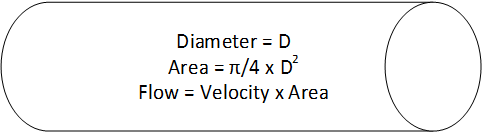
\includegraphics[scale=0.4]{PipeFlow}\\
\vspace{0.3cm}
$Flow \enspace(\mathrm{Q}) \enspace = Velocity \enspace(\mathrm{V})  \times Area \enspace(\mathrm{A})$\\
\vspace{0.2cm}
As the velocity is given in ft/min, and the area can be calculated in ft$^2$, flow can be calulated in ft$^3$/min and then converted to gal/min.\\
\vspace{0.2cm}

\vspace{0.2cm}
Step 1:  Calculating area in ft${^2}$:\\
\vspace{0.2cm}
$Area \enspace (ft^2)= \dfrac{\pi}{4}*D^2= 0.785*\Big(\dfrac{18}{12}\Big)^2 \enspace ft^2=0.785*\dfrac{324}{144}=0.349 \enspace ft^2$\\
\vspace{0.2cm}

Step 2: Calculate flow in ft$^3$/min:\\

$ Q \enspace ft^3/min = 125 \dfrac{ft}{min}*1.77 \enspace ft^2 = 221.25 \dfrac{ft^3}{min}$\\

\vspace{0.2cm}

Step 3: Convert Q to gallons per minute

\vspace{0.2cm}

$Q=221.25 \dfrac{\cancel{ft^3}}{min}*7.48\dfrac{gal}{\cancel{ft^3}}=\boxed{1655 \dfrac{gal}{min}}$


\item The velocity in a pipeline is 2 ft./sec. and the flow is 3,000 gpm. What is the diameter of the pipe in inches?

Solution:\\
\vspace{0.3cm}
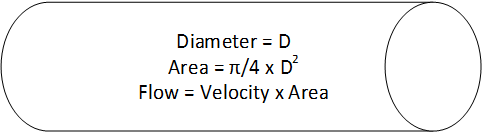
\includegraphics[scale=0.4]{PipeFlow}\\
\vspace{0.3cm}

$Flow \enspace(\mathrm{Q})= Velocity \enspace(\mathrm{V})  \times Area \enspace(\mathrm{A}) \implies Q=V*A \implies A=\dfrac{Q}{V}$\\
We need to convert Q which is given in gpm to ft${^3}$/sec and calculate the area of the pipe in ft${^2}$ given the velocity.\\
From the calculated area of the pipe, the pipe diameter can be calculated.\\
\vspace{0.2cm}
$ A \dfrac{ft}{sec} = \dfrac{Q \enspace \dfrac{\cancelto{ft^2}{ft^3}}{\cancel{sec}}}{V \enspace \dfrac{\cancelto{}{ft}}{\cancel{sec}}}$\\
\vspace{0.2cm}
Step 1 - Converting Q - 3000 gpm to ft${^3}$/sec:\\
\vspace{0.2cm}
$\dfrac{3000 \enspace \cancel{gallons}}{\bcancel{min}}*\dfrac{ft^3}{7.48 \enspace \cancel{gallon}}*\dfrac{\bcancel{min}}{60 \enspace sec}=6.68\dfrac{ft^3}{sec}$\\
\vspace{0.2cm}
Step 2 - Calculating area in ft${^2}$:\\
\vspace{0.2cm}
$\implies A \enspace ft^2 = \dfrac{ 6.68 ft^3/sec}{2 \dfrac{ft}{sec}} = 3.34 ft^2$\\
\vspace{0.3cm} 
$Area \enspace (A)= \dfrac{\pi}{4}*D^2 = 0.785*D^2 \implies D^2=\dfrac{A}{0.785} \implies D=\Big(\dfrac{A }{0.785}\Big)^{\dfrac{1}{2}}$\\
$\implies D=\Big(\dfrac{3.34}{0.785}\Big)^{\dfrac{1}{2}}=\boxed{2 \enspace ft}$\\
\vspace{0.2cm}

\item Find the flow in a 4-inch pipe when the velocity is $1.5$ feet per second.

Solution:\\
$Flow \enspace(\mathrm{Q}) \enspace = Velocity \enspace(\mathrm{V})  \times Area \enspace(\mathrm{A})$\\
\vspace{0.2cm}
The velocity is given in ft/sec and after calculating the area in ft$^2$, flow can be calculated in ft$^3$/min.\\
\vspace{0.2cm}

\vspace{0.2cm}
Step 1:  Calculating area in ft${^2}$:\\
\vspace{0.2cm}
$Area \enspace (ft^2)= \dfrac{\pi}{4}*D^2= 0.785*\Big(\dfrac{4}{12}\Big)^2 \enspace ft^2=0.785*\dfrac{324}{144}=0.087 \enspace ft^2$\\
\vspace{0.2cm}

Step 2: Calculate flow in ft$^3$/min:\\

$ Q \enspace ft^3/min = 1.5 \dfrac{ft}{sec}*0.087 \enspace ft^2 = 0.13 \dfrac{ft^3}{sec}$\\

\vspace{0.2cm}

Q can be converted to a more commonly used gallons per minute unit

\vspace{0.2cm}

$Q=0.13 \dfrac{\cancel{ft^3}}{sec}*7.48\dfrac{gal}{\cancel{ft^3}}*60\dfrac{sec}{\cancel{min}}=\boxed{59 \dfrac{gal}{min}}$
  

  \item A 42-inch diameter pipe transfers 35 cubic feet of water per second. Find the velocity in $\mathrm{ft} / \mathrm{sec}$. 

  Solution:\\
\vspace{0.3cm}
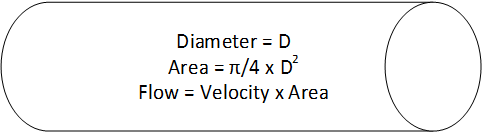
\includegraphics[scale=0.4]{PipeFlow}\\
\vspace{0.3cm}

$Flow \enspace(\mathrm{Q})= Velocity \enspace(\mathrm{V})  \times Area \enspace(\mathrm{A}) \implies Q=V*A \implies V=\dfrac{Q}{A}$\\
Q is already given in ft${^3}$/sec.  We need to first calculate the area of the pipe in ft${^2}$ so velocity can be valculated in ft/sec.\\
\vspace{0.2cm}
$ V \dfrac{ft}{sec} = \dfrac{Q \enspace \dfrac{\cancelto{ft}{ft^3}}{sec}}{A \enspace\cancel{ft^2}}$\\
\vspace{0.2cm}
Step 1 - Calculating area in ft${^2}$:\\
\vspace{0.2cm}
$Area \enspace ft^2= \dfrac{\pi}{4}*D^2= 0.785*\Big(\dfrac{42}{12}\Big)^2 \enspace ft^2=0.785*\dfrac{1764}{144}=9.616 \enspace ft^2$\\
\vspace{0.2cm}
$\implies V \dfrac{ft}{sec} = \dfrac{ 35 ft^3/sec}{9.616 \enspace ft^2} = \boxed{3.6 ft/sec}$\\
\vspace{0.3cm} 

  
  \item A plastic float is dropped into a channel and is found to travel 10 feet in $4.2$ seconds. The channel is $2.4$ feet wide and the water is flowing $1.8$ feet deep. Calculate the flow rate of water in cfs.\\
  \vspace{0.2cm}
  Solution:\\
  
  \vspace{0.2cm}
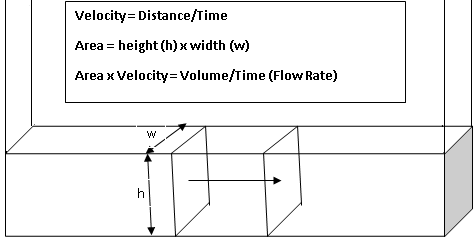
\includegraphics[scale=0.4]{ChannelFlow3}\\
$Q=V*A \implies V=\dfrac{Q}{A}$\\
\vspace{0.3cm}
  $Flow \enspace(\mathrm{Q})= Velocity \enspace(\mathrm{V})  \times Area \enspace(\mathrm{A})$\\

The speed of the float travelling is the velocity of the water $\implies Velocity = \dfrac{10 \enspace ft}{4.2 \enspace sec}$

Thus flow = $\dfrac{10 \enspace ft}{4.2 \enspace sec} * (2.4*1.8) ft^2 = \boxed{4.32 \dfrac{ft^3}{sec}} $\\

\vspace{0.2cm}

\item A channel is 3.25 feet wide and is conveying a a flow of 3.5 MGD. The depth of the water is 8 inches. Calculate the velocity of this flow.\\
Solution:\\
\vspace{0.2cm}
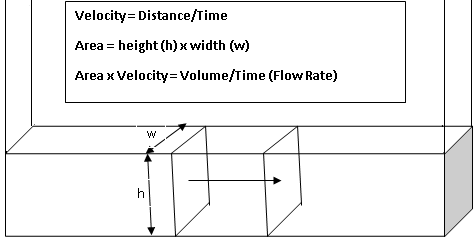
\includegraphics[scale=0.4]{ChannelFlow3}\\
$Q=V*A \implies V=\dfrac{Q}{A}$\\
\vspace{0.3cm}
$\implies V\dfrac{ft}{s}=\dfrac{3.5\dfrac{\cancel{MG}}{\cancel{day}}*\dfrac{1000000\cancel{gal}}{\cancel{MG}}*\dfrac{ft^{\cancel{3}}}{7.48\cancel{gal}}*\dfrac{\cancel{day}}{(1440*60)s}}{(3.25*0.75)\cancel{ft^2}}=\boxed{2.2\dfrac{ft}{s}}$

\end{enumerate}
\section*{Practice Problems - Unit Conversions} \index{Math solutions! Unit Conversions}
\begin{enumerate}

\item Convert 1000 $ft^3$ to cu. yards\\
Solution:\\
\vspace{0.2cm}
$yds^3=1000ft^3*\dfrac{yd^3}{27 \enspace ft^3}=\boxed{37 \enspace yds^3}$\\
\vspace{0.2cm}

\item Convert 10 gallons/min to $ft^3$/hr\\
Solution:\\
\vspace{0.2cm}
$\dfrac{ft^3}{hr}=10\dfrac{\cancel{gal}}{\cancel{min}}*\dfrac{ft^3}{7.48\cancel{gal}}*\dfrac{60\cancel{min}}{hr}=\boxed{80.2 \dfrac{ft^3}{hr}}$
\vspace{0.2cm}

\item Find the flow in gpm when the flow is $0.25 \mathrm{cfs}$.\\
Solution:\\
\vspace{0.2cm}
$\dfrac{gal}{min}=0.25\dfrac{\cancel{ft^3}}{\cancel{sec}}*\dfrac{7.48gal}{\cancel{ft^3}}*\dfrac{60\cancel{sec}}{min}=\boxed{112.2 \dfrac{gal}{min}}$
vspace{0.2cm}

\item The flow rate through a filter is 4.25 MGD. What is this flow rate expressed as gpm?\\
Solution:\\
\vspace{0.2cm}
$\dfrac{gal}{min}=4.25\dfrac{\cancel{MG}}{\cancel{day}}*\dfrac{1,000,000gal}{\cancel{MG}}*\dfrac{\cancel{day}}{1,440min}=\boxed{2,951 \dfrac{gal}{min}}$
\vspace{0.2cm}

\item After calibrating a chemical feed pump, you've determined that the maximum feed rate is $178 \mathrm{~mL} /$ minute. If this pump ran continuously, how many gallons will it pump in a full day?\\
Solution:\\
\vspace{0.2cm}
$\dfrac{gal}{day}=178\dfrac{\cancel{mL}}{\cancel{min}}*\dfrac{L}{1000\cancel{mL}}*\dfrac{1,440\cancel{min}}{day}=\boxed{119,680 \dfrac{gal}{day}}$


\vspace{0.2cm}
\item A plant produces 2,000 cubic foot of water per hour. How many gallons of water is produced in an 8-hour shift?\\
Solution:\\
\vspace{0.2cm}
$\dfrac{gal}{8-hr \enspace shift}=2,000\dfrac{\cancel{ft^3}}{\cancel{hr}}*\dfrac{7.48gal}{\cancel{ft^3}}*\dfrac{8\cancel{hr}}{8-hr \enspace shift}=\boxed{253.6 \dfrac{gal}{day}}$
\vspace{0.2cm}

\item Change 70 °F to °C\\
Solution:\\
\vspace{0.2cm}
$\degree{C} = \dfrac{\degree{F}-32}{1.8} = \dfrac{70-32}{1.8}=\boxed{21.1\degree{C}}$
\vspace{0.2cm}

\item Change 4 °C to °F\\
Solution:\\
\vspace{0.2cm}
$\degree{F}=(\degree{C} \times 1.8)+32 = (4*1.8)+32=\boxed{39.2\degree{F}}$
\vspace{0.2cm}
\end{enumerate}


\section*{Practice Problems - Concentration} \index{Math solutions! Concentration}
\begin{enumerate}
\item What is the concentration in mg/l of  4.5\% solution of that substance.\\
$\boxed{450,000mg/l}$
\vspace{0.3cm}
\item How many lbs of salt needs to be dissolved in water to make 1 liter of 5\% salt solution?\\
Solution:\\
$5\% \enspace salt \enspace solution \enspace \implies 50,000 \enspace mg/l \enspace salt$\\
To prepare 1 litre of salt solution need to dissolve 50,000 mg or:\\
$50,000 \enspace mg*\dfrac{lb}{453.6 \enspace gms}*\dfrac{gm}{1,000 \enspace mg}=\boxed{0.11 \enspace lb \enspace salt}\enspace$in enough  water to make 1 liter of solution.\\
\vspace{0.3cm}
\item An operator mixes 40 lb of lime in a 100-gal tank containing 80 gal of water. What is the percent of lime in the slurry?\\
\vspace{0.2cm}
Solution:\\
\vspace{0.2cm}
$\Bigg(\dfrac{40 \enspace lbs \enspace lime}{80 \enspace gal \enspace water*8.34\dfrac{lbs}{gal \enspace water}+40\enspace lbs \enspace lime}*\dfrac{1,000,000 \enspace lbs}{million \enspace lbs}\Bigg)ppm*\dfrac{\%}{10,000 \enspace ppm}$\\
\vspace{0.2cm}
$=\boxed{5.7\%}$


\end{enumerate}

\section*{Practice Problems - Density and Specific Gravity} \index{Math solutions! Density and specific gravity}
\begin{enumerate}

\item What is the specific gravity of a 1 ft$^3$ concrete block which weighs 145 lbs?
Solution:\\
Specific gravity is the ratio of the weight of the substance to that of an equal volume of water.\\
As one cu. ft of water weighs 62.43 lbs/cu. ft (8.34 lbs/gal*7.48 gal/cu. ft):\\
Specific gracvity of this concrete block=$\dfrac{145}{62.43}=\boxed{2.3}$
\vspace{0.2cm}

\item What is the specific gravity of a chlorine solution if 1 (one) gallon weighs 10.2lbs?
Solution:\\
\vspace{0.2cm}
Specific gravity is the ratio of the weight of the substance to that of an equal volume of water.\\
As one gallon of water weighs 8.34 lbs: Specific gracvity of this chlorine solution=$\dfrac{10.2}{8.34}=\boxed{1.2}$
\vspace{0.2cm}




\item How much does each gallon of zinc orthophosphate weigh (pounds) if it has a specific gravity of 1.46?\\
\vspace{0.2cm}
Solution:\\
\vspace{0.2cm}
$8.34\dfrac{lb}{gal}*1.46=\boxed{12.18\dfrac{lb}{gal}}$
\vspace{0.2cm}
\item How much does a 55 gallon drum of 25\% caustic soda weigh (pounds) if the specific gravity is 1.28?\\
\vspace{0.2cm}
Solution:\\
\vspace{0.2cm}
$8.34\dfrac{lb}{\cancel{gal}}*1.28*55\cancel{gal}=\boxed{12.18\dfrac{lb}{gal}}$
\vspace{0.2cm}
\end{enumerate}


\section*{Practice Problems - Pounds Formula} \index{Math solutions! Pounds formula}
\begin{enumerate}

\item A water treatment plant operates at the rate of 75 gallons per minute. They dose soda ash at 14 mg/L. How many pounds of soda ash will they use in a day?
\\

\begin{figure}[h]
\begin{tikzpicture}
    \newcommand{\R}{1.5}

\path[help lines,step=.2] (0,0) grid (16,3);
\path[help lines,line width=.6pt,step=1] (0,0) grid (16,3);
%\foreach \x in {0,1,2,3,4,5,6,7,8,9,10,11,12,13,14,15,16}
%\node[anchor=north] at (\x,0) {\x};
%\foreach \y in {0,1,2,3,4,5,6}
%\node[anchor=east] at (0,\y) {\y};
%-------------CIRCLE-----------------------------------
\draw[black,fill=gray!10] (8,3) circle (\R);
\draw[black, very thick, rotate=0](6.5,3) -- (9.5,3);
\draw (8,3.6) node[text width=3cm,align=center]
  {\scriptsize{lbs/day}};
\draw (7.1,2.5) node[text width=3cm,align=center]
  {\tiny{14 mg/l}};
\draw (8.9,2.5) node[text width=3cm,align=center]
  {\tiny{75 GPM}};
  \draw (8,2)node[text width=3cm,align=center]
  {\tiny{8.34}};
\draw[black, very thick, rotate=0](7.2,1.7) -- (8,3);
\draw[black, very thick, rotate=0](8.8,1.7) -- (8,3);
\end{tikzpicture}
\end{figure}
$\dfrac{\mathrm{lbs}}{\mathrm{day}}=\mathrm{Flow}\dfrac{{\mathrm{MG}}}{\mathrm{day}}* \mathrm{Concentration}\dfrac{\mathrm{mg}}{\mathrm{l}}*8.34$
\\
\vspace{0.2cm}
$\dfrac{\mathrm{lbs}}{\mathrm{day}}=75 \dfrac{\cancel{\mathrm{gallons}}}{\cancel{\mathrm{min}}}* 1440\dfrac{\cancel{\mathrm{min}}}{\mathrm{day}}*\dfrac{\mathrm{MG}}{1,000,000 \enspace \cancel{\mathrm{gallons}}}*250\dfrac{\mathrm{mg}}{\mathrm{l}}*8.34 = \boxed{225\dfrac{lbs}{day}}$
\vspace{0.2cm}


\item What is the influent plant loading of phosphorus in lbs/day if the plant flow is 4.5 MGD and the influent phosphorous concentration is 1.5 mg/l?\\
\vspace{0.2cm}
Solution:\\
\vspace{0.2cm}
 \begin{figure}[h!]
\begin{tikzpicture}
    \newcommand{\R}{1.5}

\path[help lines,step=.2] (0,0) grid (16,3);
\path[help lines,line width=.6pt,step=1] (0,0) grid (16,3);
%\foreach \x in {0,1,2,3,4,5,6,7,8,9,10,11,12,13,14,15,16}
%\node[anchor=north] at (\x,0) {\x};
%\foreach \y in {0,1,2,3,4,5,6}
%\node[anchor=east] at (0,\y) {\y};
%-------------CIRCLE-----------------------------------
\draw[black,fill=gray!10] (8,3) circle (\R);
\draw[black, very thick, rotate=0](6.5,3) -- (9.5,3);
\draw (8,3.6) node[text width=3cm,align=center]
  {\scriptsize{? lbs/day}};
\draw (7.1,2.5) node[text width=3cm,align=center]
  {\tiny{1.5 mg/l}};
\draw (8.9,2.5) node[text width=3cm,align=center]
  {\tiny{4.5 MGD}};
  \draw (8,2)node[text width=3cm,align=center]
  {\tiny{8.34}};
\draw[black, very thick, rotate=0](7.2,1.7) -- (8,3);
\draw[black, very thick, rotate=0](8.8,1.7) -- (8,3);
\end{tikzpicture}
\end{figure}


\vspace{0.2cm}
$1.5\dfrac{mg}{l}*4.5MGD*8.34=\boxed{56 \enspace lbs/day}$\\
\vspace{0.2cm}

\item A water treatment plant uses 8 pounds of chlorine daily and the dose is 17 mg/l. How
many gallons are they producing?
\vspace{0.2cm}
Solution:\\
\vspace{0.2cm}
 \begin{figure}[h!]
\begin{tikzpicture}
    \newcommand{\R}{1.5}

\path[help lines,step=.2] (0,0) grid (16,3);
\path[help lines,line width=.6pt,step=1] (0,0) grid (16,3);
%\foreach \x in {0,1,2,3,4,5,6,7,8,9,10,11,12,13,14,15,16}
%\node[anchor=north] at (\x,0) {\x};
%\foreach \y in {0,1,2,3,4,5,6}
%\node[anchor=east] at (0,\y) {\y};
%-------------CIRCLE-----------------------------------
\draw[black,fill=gray!10] (8,3) circle (\R);
\draw[black, very thick, rotate=0](6.5,3) -- (9.5,3);
\draw (8,3.6) node[text width=3cm,align=center]
  {\scriptsize{8 lbs/day}};
\draw (7.1,2.5) node[text width=3cm,align=center]
  {\tiny{17 mg/l}};
\draw (8.9,2.5) node[text width=3cm,align=center]
  {\tiny{? MGD}};
  \draw (8,2)node[text width=3cm,align=center]
  {\tiny{8.34}};
\draw[black, very thick, rotate=0](7.2,1.7) -- (8,3);
\draw[black, very thick, rotate=0](8.8,1.7) -- (8,3);
\end{tikzpicture}
\end{figure}
$\dfrac{\mathrm{lbs}}{\mathrm{day}}=\mathrm{Flow}\dfrac{{\mathrm{MG}}}{\mathrm{day}}* \mathrm{Concentration}\dfrac{\mathrm{mg}}{\mathrm{l}}*8.34 \hspace{0.2cm}$\\
\vspace{0.2cm}
$\implies \mathrm{Flow}\dfrac{{\mathrm{MG}}}{day}=\dfrac{ \dfrac{\mathrm{lbs}}{\mathrm{day}}}{\mathrm{Concentration}\dfrac{\mathrm{mg}}{\mathrm{l}}*8.34}=\dfrac{8 \dfrac{\mathrm{lbs}}{\mathrm{day}}}{17\dfrac{\mathrm{mg}}{\mathrm{l}}*8.34}=0.056425\dfrac{{\mathrm{MG}}}{day}$\\
\vspace{0.2cm}
$0.056425\dfrac{{\mathrm{MG}}}{day}*\dfrac{1,000,000 \enspace \mathrm{Gallons}}{\mathrm{MG}}=\boxed{56,425 \enspace \mathrm{Gallons}}$
\vspace{0.2cm}





\end{enumerate}








\section*{Practice Problems - Chemical Dosing} \index{Math solutions! Chemical dosing}
\begin{enumerate}

\item In order to disinfect a sedimentation basin measuring $20 \mathrm{ft}$ in width, 60 feet in length, and is 10 feet deep to obtain $50 \mathrm{ppm}$ would require how many lbs. of $65 \%$ available $\mathrm{HTH}$ ?\\
a) $5.0 \mathrm{lbs}$\\
b) $41.3 \mathrm{lbs}$\\
c) $37.4 \mathrm{lbs}$\\
*d) $57.6 \mathrm{lbs}$\\

\item Determine the chlorinator setting (lb/day) required to treat a flow of $4 \mathrm{MGD}$ with a chlorine dose of $5 \mathrm{mg} / \mathrm{L}$.

Chlorine feed rate $(\mathrm{lb} /$ day $)=$ Chlorine $(\mathrm{mg} / \mathrm{L}) \times$ Flow $(\mathrm{MGD}) \times 8.34 \mathrm{lb} / \mathrm{gal}$

Chlorine feed rate $(\mathrm{lb} /$ day $)=5 \mathrm{mg} / \mathrm{L} \times 4 \mathrm{MGD} \times 8.34 \mathrm{lb} / \mathrm{gal}$

Chlorine feed rate $(\mathrm{lb} /$ day $)=167 \mathrm{lb} /$ day

\item A pipeline that is 12 inches in diameter and $1400 \mathrm{ft}$ long is to be treated with a chlorine dose of $48 \mathrm{mg} / \mathrm{L}$. How many lb of chlorine will this require?

First determine the gallon volume of the pipeline:

Volume $(\mathrm{gal})=0.785 \times \mathrm{D}^{2} \times$ length $(\mathrm{ft}) \times 7.48 \mathrm{gal} / \mathrm{cu} \mathrm{ft}$

Volume $(\mathrm{gal})=0.785 \times(1 \mathrm{ft})^{2} \times 1400 \mathrm{ft} \times 7.48 \mathrm{gal} / \mathrm{cu} \mathrm{ft}$ Volume $(\mathrm{gal})=8221 \mathrm{gal}$

Next calculate the amount of chlorine required:

Chlorine feed rate $(\mathrm{lb} /$ day $)=$ Chlorine $(\mathrm{mg} / \mathrm{L})$ x Flow $($ MGD) $\times 8.34 \mathrm{lb} / \mathrm{gal}$

Chlorine feed rate $(\mathrm{lb} /$ day $)=48 \mathrm{mg} / \mathrm{L} \times 0.008221 \mathrm{MGD} \times 8.34 \mathrm{lb} / \mathrm{gal}$

Chlorine feed rate $(\mathrm{lb} /$ day $)=3.3 \mathrm{lb}$

\item What should the chlorinator seting be (lb/day) to treat a flow of $2.35 \mathrm{MGD}$ if the chlorine demand is $3.2 \mathrm{mg} / \mathrm{L}$ and a chlorine residual of $0.9 \mathrm{mg} / \mathrm{L}$ is desired?

First, determine the chlorine dosage (in $\mathrm{mg} / \mathrm{L}$ ):

Chlorine Dose $(\mathrm{mg} / \mathrm{L})=$ Chlorine Demand $+$ Chlorine Residual

Chlorine Dose $(\mathrm{mg} / \mathrm{L})=3.2 \mathrm{mg} / \mathrm{L}+0.9 \mathrm{mg} / \mathrm{L}$

Chlorine Dose $(\mathrm{mg} / \mathrm{L})=4.1 \mathrm{mg} / \mathrm{L}$

Next calculate the chlorine dosage (feed rate) in $\mathrm{lb} /$ day:

Chlorine feed rate $(\mathrm{lb} /$ day $)=$ Chlorine $(\mathrm{mg} / \mathrm{L}) \times$ Flow $(\mathrm{MGD}) \times 8.34 \mathrm{lb} / \mathrm{gal}$

Chlorine feed rate $(\mathrm{lb} /$ day $)=4.1 \mathrm{mg} / \mathrm{L} \times 2.35 \mathrm{MGD} \times 8.34 \mathrm{lb} / \mathrm{gal}$

Chlorine feed rate $(\mathrm{lb} /$ day $)=80.4 \mathrm{lb} /$ day

\item A water treatment plant operates at the rate of 75 gallons per minute. They dose soda ash at 14 mg/L. How many pounds of soda ash will they use in a day?
Solution:\\
\vspace{0.2cm}
\begin{figure}[h]
\begin{tikzpicture}
    \newcommand{\R}{1.5}

\path[help lines,step=.2] (0,0) grid (16,3);
\path[help lines,line width=.6pt,step=1] (0,0) grid (16,3);
%\foreach \x in {0,1,2,3,4,5,6,7,8,9,10,11,12,13,14,15,16}
%\node[anchor=north] at (\x,0) {\x};
%\foreach \y in {0,1,2,3,4,5,6}
%\node[anchor=east] at (0,\y) {\y};
%-------------CIRCLE-----------------------------------
\draw[black,fill=gray!10] (8,3) circle (\R);
\draw[black, very thick, rotate=0](6.5,3) -- (9.5,3);
\draw (8,3.6) node[text width=3cm,align=center]
  {\scriptsize{lbs/day}};
\draw (7.1,2.5) node[text width=3cm,align=center]
  {\tiny{14 mg/l}};
\draw (8.9,2.5) node[text width=3cm,align=center]
  {\tiny{75 GPM}};
  \draw (8,2)node[text width=3cm,align=center]
  {\tiny{8.34}};
\draw[black, very thick, rotate=0](7.2,1.7) -- (8,3);
\draw[black, very thick, rotate=0](8.8,1.7) -- (8,3);
\end{tikzpicture}
\end{figure}
$\dfrac{\mathrm{lbs}}{\mathrm{day}}=\mathrm{Flow}\dfrac{{\mathrm{MG}}}{\mathrm{day}}* \mathrm{Concentration}\dfrac{\mathrm{mg}}{\mathrm{l}}*8.34$
\\
\vspace{0.2cm}
$\dfrac{\mathrm{lbs}}{\mathrm{day}}=75 \dfrac{\cancel{\mathrm{gallons}}}{\cancel{\mathrm{min}}}* 1440\dfrac{\cancel{\mathrm{min}}}{\mathrm{day}}*\dfrac{\mathrm{MG}}{1,000,000 \enspace \cancel{\mathrm{gallons}}}*14\dfrac{\mathrm{mg}}{\mathrm{l}}*8.34 = \boxed{12.6\dfrac{lbs}{day}}$
\vspace{0.2cm}

\item A water treatment plant is producing 1.5 million gallons per day of potable water, and uses 38 pounds of soda ash for pH adjustment. What is the dose of soda ash at that plant?\\
Solution:\\
 \begin{figure}[h!]
\begin{tikzpicture}
    \newcommand{\R}{1.5}

\path[help lines,step=.2] (0,0) grid (16,3);
\path[help lines,line width=.6pt,step=1] (0,0) grid (16,3);
%\foreach \x in {0,1,2,3,4,5,6,7,8,9,10,11,12,13,14,15,16}
%\node[anchor=north] at (\x,0) {\x};
%\foreach \y in {0,1,2,3,4,5,6}
%\node[anchor=east] at (0,\y) {\y};
%-------------CIRCLE-----------------------------------
\draw[black,fill=gray!10] (8,3) circle (\R);
\draw[black, very thick, rotate=0](6.5,3) -- (9.5,3);
\draw (8,3.6) node[text width=3cm,align=center]
  {\scriptsize{38 lbs/day}};
\draw (7.1,2.5) node[text width=3cm,align=center]
  {\tiny{? mg/l}};
\draw (8.9,2.5) node[text width=3cm,align=center]
  {\tiny{1.5 MGD}};
  \draw (8,2)node[text width=3cm,align=center]
  {\tiny{8.34}};
\draw[black, very thick, rotate=0](7.2,1.7) -- (8,3);
\draw[black, very thick, rotate=0](8.8,1.7) -- (8,3);
\end{tikzpicture}
\end{figure}
$\dfrac{\mathrm{lbs}}{\mathrm{day}}=\mathrm{Flow}\dfrac{{\mathrm{MG}}}{\mathrm{day}}* \mathrm{Concentration}\dfrac{\mathrm{mg}}{\mathrm{l}}*8.34 \hspace{0.2cm} \implies \mathrm{Concentration}\dfrac{\mathrm{mg}}{\mathrm{l}}=\dfrac{ \dfrac{\mathrm{lbs}}{\mathrm{day}}}{\mathrm{Flow}\dfrac{{\mathrm{MG}}}{\mathrm{day}}*8.34}$
\vspace{0.2cm}
$\mathrm{Concentration}\dfrac{\mathrm{mg}}{\mathrm{l}}=\dfrac{ 38\dfrac{\mathrm{lbs}}{\mathrm{day}}}{1.5\dfrac{{\mathrm{MG}}}{\mathrm{day}}*8.34}=\boxed{3\dfrac{\mathrm{mg}}{\mathrm{l}}}$
\\
\vspace{0.2cm}


\item A water treatment plant produces 150,000 gallons of water every day. It uses an average of 2 pounds of permanganate for iron and manganese removal. What is the dose of the permanganate? \\
 Solution:\\
 \vspace{0.2cm}
 \begin{figure}[h!]
\begin{tikzpicture}
    \newcommand{\R}{1.5}

\path[help lines,step=.2] (0,0) grid (16,3);
\path[help lines,line width=.6pt,step=1] (0,0) grid (16,3);
%\foreach \x in {0,1,2,3,4,5,6,7,8,9,10,11,12,13,14,15,16}
%\node[anchor=north] at (\x,0) {\x};
%\foreach \y in {0,1,2,3,4,5,6}
%\node[anchor=east] at (0,\y) {\y};
%-------------CIRCLE-----------------------------------
\draw[black,fill=gray!10] (8,3) circle (\R);
\draw[black, very thick, rotate=0](6.5,3) -- (9.5,3);
\draw (8,3.6) node[text width=3cm,align=center]
  {\scriptsize{38 lbs/day}};
\draw (7.1,2.5) node[text width=3cm,align=center]
  {\tiny{? mg/l}};
\draw (8.9,2.5) node[text width=3cm,align=center]
  {\tiny{1.5 MGD}};
  \draw (8,2)node[text width=3cm,align=center]
  {\tiny{8.34}};
\draw[black, very thick, rotate=0](7.2,1.7) -- (8,3);
\draw[black, very thick, rotate=0](8.8,1.7) -- (8,3);
\end{tikzpicture}
\end{figure}
$\dfrac{\mathrm{lbs}}{\mathrm{day}}=\mathrm{Flow}\dfrac{{\mathrm{MG}}}{\mathrm{day}}* \mathrm{Concentration}\dfrac{\mathrm{mg}}{\mathrm{l}}*8.34 \hspace{0.2cm} \implies \mathrm{Concentration}\dfrac{\mathrm{mg}}{\mathrm{l}}=\dfrac{ \dfrac{\mathrm{lbs}}{\mathrm{day}}}{\mathrm{Flow}\dfrac{{\mathrm{MG}}}{\mathrm{day}}*8.34}$
\vspace{0.2cm}
$\mathrm{Concentration}\dfrac{\mathrm{mg}}{\mathrm{l}}=
\dfrac{ 2\dfrac{\mathrm{lbs}}{\mathrm{day}}}
{\Bigg(150,000 \dfrac{\cancel{\mathrm{Gallons}}}
{\mathrm{day}}*
\dfrac{\mathrm{MG}}
{1,000,000 \cancel{\enspace \mathrm{Gallons}}}*8.34\Bigg)}
=\boxed{3\dfrac{\mathrm{mg}}{\mathrm{l}}}$

\end{enumerate}


\section*{Practice Problems - Blending and Dilution} \index{Math solutions! Blending and dilution}


\vspace{0.2cm}
\begin{enumerate}
\item Ferric chloride is being added as a coagulant to the raw water entering a plant. Sampling shows that the concentration of ferric in the raw water is 25 ppm. A quick check of the chemical metering pump shows that it is operating at a flow rate of 4.3 gpm. If the flow through the water plant is 800 gpm, what is the concentration of raw chemical in the dosing tank?\\
\vspace{0.2cm}
Solution:\\
\vspace{0.3cm}
\begin{tikzpicture}

\draw [-] (-3.2,4.2) -- (-0.4,4.2);
\draw [->] (-0.2,4) -- (-0.2,1.9);
\draw [->] (-3.2,1.9) -- (4,1.9);
\draw [shift={(-0.4,4)}] plot[domain=0:1.57,variable=\t]({1*0.2*cos(\t r)+0*0.2*sin(\t r)},{0*0.2*cos(\t r)+1*0.2*sin(\t r)});
\draw (-3.1,4.1) node[anchor=north west] {V$_{\tiny{FeCl_3}}$=$4.3 gpm$};
\draw (-3.1,3.6) node[anchor=north west] {C$_{\tiny{FeCl_3}}$ = ?};
\draw (-4.2,4.5) node[anchor=north west] {FeCl$_3$};
\draw (-4.2,2.2) node[anchor=north west] {Water};
\draw (-2.1,1.8) node[anchor=north west] {$800 gpm$};
\draw (0.7,1.8) node[anchor=north west] {C$_2$=25ppm FeCl$_3$};
\draw (0.7,1.3) node[anchor=north west] {V$_2$=4.3+800=804.3 gpm};
\end{tikzpicture}\\
\vspace{0.2cm}
C$_1$ * V$_1$ = C$_2$ * V$_2$ \\
\vspace{0.2cm}
C$_{\tiny{FeCl_3}}$ * V$_{\tiny{FeCl_3}}$  =  C$_2$ * (V$_{\tiny{FeCl_3}}$+V$_{\tiny{Water}}$)\\
\vspace{0.2cm}
C$_{\tiny{FeCl_3}}$ * 4.3 =  25 * (804.3)\\
\vspace{0.2cm}
C$_{\tiny{FeCl_3}}=\dfrac{25 * (804.3)}{4.3}=\boxed{4,676 \enspace \mathrm{ppm} \enspace \mathrm{or} \enspace 0.47\%}$\\
\vspace{0.3cm}
\item A water plant is fed by two different wells. The first well produces water at a rate of 600 gpm and contains arsenic at 0.5 mg/L. The second well produces water at a rate of 350 gpm and contains arsenic at 12.5 mg/L. What is the arsenic concentration of the blended water?\\
\vspace{0.2cm}
Solution:\\
\vspace{0.2cm}
C$_1$ * V$_1$ + C$_2$ * V$_2$ + =  C$_3$ * V$_3$=C$_3$*(V$_1$ + V$_2$)\\
\vspace{0.2cm}
C$_{Well \enspace 1}$ * V$_{Well \enspace 1}$ + C$_{Well \enspace 2}$ * V$_{Well \enspace 2}$ =  C$_{Blend}$ * V$_{Blend}$=C$_{Blend}$*(V$_{Well \enspace1}$ + V$_{Well \enspace 2}$)\\
\vspace{0.3cm}
$\implies C_{Blend}=\dfrac{C_{Well \enspace 1} * V_{Well \enspace 1} + C_{Well \enspace 2} * V_{Well \enspace 2}}{V_{Well \enspace 1} + V_{Well \enspace 2}}=\dfrac{0.5*600+12.5*350}{600+350}=\boxed{4.9 \enspace \textrm{mg/l}}$
\end{enumerate}

\section*{Practice Problems - Pumping Rates} \index{Math solutions!Pumping rates}

\begin{enumerate}
\item How long will it take (hrs) to fill a 2 ac-ft pond if the pumping rate is 400 GPM?\\

 
 \vspace{0.2cm}
 
 $Time \enspace to \enspace fill \enspace(hours)= \dfrac{Volume}{Flow}=\dfrac{2 \enspace \cancel{Ac-ft}*\dfrac{325,851 \enspace \cancel{gallons}}{\cancel{Ac-ft}}}{400 \dfrac{\cancel{gallons}}{\cancel{min}}*\dfrac{60 \enspace\cancel{ min}}{hr}}=\boxed{27 \enspace hours}$\\
 
\item A pump is set to pump 5 minutes each hour. It pumps at the rate of 35 gpm. How many gallons of water are pumped each day?\\
Solution:\\
$\dfrac{35 \enspace gal \enspace sludge}{\cancel{min}}*\dfrac{5 \enspace \cancel{min}}{\cancel{hr}} *\dfrac{24 \enspace \cancel{hr}}{day}=\boxed{\dfrac{4,200 \enspace gallons}{day}}$\\
\vspace{0.5cm}

\item A pump operates 5 minutes each 15 minute interval.  If the pump capacity is 60 gpm, how many gallons are pumped daily?\\

$\dfrac{60 \enspace gal \enspace sludge}{\xcancel{min}}*\dfrac{5 \enspace \xcancel{min}}{15 \enspace \cancel{min}}*1440\dfrac{\cancel{min}}{day}=\boxed{\dfrac {28,800 \enspace gal \enspace sludge }{day}}$\\
\vspace{0.5cm}

\item Given the tank is 10ft wide, 12 ft long and 18 ft deep tank including 2 ft of freeboard when filled to capacity. How much time (minutes) will be required to pump down this tank to a depth of 2 ft when the tank is at maximum capacity using a 600 GPM pump\\
Solution:\\
\vspace{0.5cm}


\begin{tikzpicture}

\pgfmathsetmacro{\cubexx}{4}
\pgfmathsetmacro{\cubeyy}{1.5}
\pgfmathsetmacro{\cubezz}{2}
\pgfmathsetmacro{\cubex}{4}
\pgfmathsetmacro{\cubey}{0.5}
\pgfmathsetmacro{\cubez}{2}
\pgfmathsetmacro{\cubexxx}{4}
\pgfmathsetmacro{\cubeyyy}{4}
\filldraw [fill=cyan!10!white, draw=black] (0,-\cubey,0) -- ++(-\cubexx,0,0) -- ++(0,-\cubeyy,0) -- ++(\cubexx,0,0) -- cycle ;
\filldraw [fill=cyan!0!white, draw=black] (0,-\cubey,0) -- ++(0,0,-\cubezz) -- ++(0,-\cubeyy,0) -- ++(0,0,\cubezz) -- cycle;
\filldraw [fill=cyan!10!white, draw=black] (0,-\cubey,0) -- ++(0,0,-\cubezz) -- ++(0,-\cubeyy,0) -- ++(0,0,\cubezz) -- cycle;
%\filldraw [fill=cyan!10!white, draw=black] (0,-\cubey,0) -- ++(-\cubexx,0,0) -- ++(0,0,-\cubezz) -- ++(\cubexx,0,0) -- cycle;
%%%\draw (0,-0.5,0) -- ++(-\cubex,0,0) -- ++(0,-\cubey,-\cubez) -- ++(\cubex,0,0) -- cycle;
\draw (-\cubex,0,0) -- ++(0,0,-\cubez) -- ++(0,-\cubey,0) -- ++(0,0,\cubez) -- cycle;
\draw (0,-\cubey,0) -- ++(-\cubex,0,0) -- ++(0,0,-\cubez) -- ++(\cubex,0,0) -- cycle;
\filldraw [fill=white, draw=black] (0,0,0) -- ++(-\cubex,0,0) -- ++(0,-\cubey,0) -- ++(\cubex,0,0) -- cycle ;
\filldraw [fill=white, draw=black] (0,0,0) -- ++(0,0,-\cubez) -- ++(0,-\cubey,0) -- ++(0,0,\cubez) -- cycle;
\filldraw [fill=white, draw=black] (0,0,0) -- ++(0,0,-\cubez) -- ++(0,-\cubey,0) -- ++(0,0,\cubez) -- cycle;
\filldraw [fill=white, draw=black] (0,0,0) -- ++(-\cubex,0,0) -- ++(0,0,-\cubez) -- ++(\cubex,0,0) -- cycle;

%\filldraw [fill=RoyalBlue!10!white, draw=black] (0,-1.5,0) -- ++(-\cubex,0,0) -- ++(0,-\cubey,0) -- ++(\cubex,0,0) -- cycle ;

%\filldraw [fill=RoyalBlue!10!white, draw=black] (0,-1.5,0) -- ++(0,0,-\cubez) -- ++(0,-\cubey,0) -- ++(0,0,\cubez) -- cycle;



%%\draw (0,-0.5,0) -- ++(-\cubex,0,0) -- ++(0,0,-\cubez) -- ++(\cubex,0,0) -- cycle;
%%\filldraw [fill=white, draw=black] (-\cubex,0,0) -- ++(0,0,-\cubez) -- ++(0,-\cubey,0) -- ++(0,0,\cubez) -- cycle;
%%\filldraw [fill=white, draw=black] (0,-\cubey,0) -- ++(-\cubex,0,0) -- ++(0,0,-\cubez) -- ++(\cubex,0,0) -- cycle ;

\draw [<->] (-4,-2.3) -- (0,-2.3) node [midway, below] {12' Long};
\draw [<->] (1,-1.3) -- (1,.2) node [midway, midway] {\hspace{4.5cm}16' Water Depth (Initial)};
\draw [<->] (0.4,-1.62) -- (0.4,-1.1) node [midway, midway] {\hspace{-4.8cm} 2' Water Depth (Final)};
\draw [<->] (1,.8) -- (1,.2) node [midway, midway] {\hspace{2.4cm}2' Freeboard};
\draw [<->] (1,-1.3) -- (0,-2.3) node [midway, midway] {\hspace{2.3cm}10' Wide};
\end{tikzpicture}\\
Volume to be pumped=$12 \enspace ft*10 \enspace ft *(16-2)\enspace ft=1,680ft^3$\\
\vspace{0.3cm}
$\implies \dfrac{1,680\cancel{ft^3}*7.48\dfrac{\cancel{gal}}{\cancel{ft^3}}}{600\dfrac{\cancel{gal}}{min}}=\boxed{21min}$

\end{enumerate}



\section*{Practice Problems - Pressure, Force and Head Relationship} \index{Math solutions! Pressure, force and head relationship}
\begin{enumerate}


\item A 42-inch main line has a shut off valve. The same line has a 10-inch bypass line with another shut-off valve. Find the amount of force on each valve if the water pressure in the line is 80 psi. Express your answer in tons.\\
\vspace{0.2cm}
Solution:\\
\vspace{0.2cm}
$\textrm{Force}= \textrm{Pressure} \times \textrm{Area}$\\
\vspace{0.3cm}
Force on the 42-in valve:
\vspace{0.3cm}
$\implies 80 \enspace \dfrac{\mathrm{lbs}}{\mathrm{in^2}}*0.785 *(42 \mathrm{in})^2*\dfrac{1 \mathrm{ton}}{2000 \mathrm{lbs}} =\boxed{3.39 \enspace\mathrm{tons}}$\\
\vspace{0.3cm}
Force on the 10-in valve:
\vspace{0.3cm}
$\implies 80 \enspace \dfrac{\mathrm{lbs}}{\mathrm{in^2}}*0.785 *(10 \mathrm{in})^2*\dfrac{1 \mathrm{ton}}{2000 \mathrm{lbs}} =\boxed{3.39 \enspace\mathrm{tons}}$
\vspace{0.2cm}
\item A water tank is 15 feet deep and 30 feet in diameter. What is the force exerted on a 6-inch valve at the bottom of the tank?\\
\vspace{0.5cm}
$\textrm{Force}= \textrm{Pressure} \times \textrm{Area}$\\
\vspace{0.5cm}
$\implies 15 \enspace\mathrm{ft}* \dfrac{0.433 \enspace \mathrm{psi}}{\mathrm{ft}}*0.785 *(6 \mathrm{in})^2 =\boxed{183 \enspace\mathrm{lbs}}$\\

\item A water tank is filled to depth of 22 feet. What is the psi at the bottom of the tank?\\
 \vspace{0.2cm}
Solution:\\ 
 \vspace{0.2cm}
$
22 \enspace \cancel{ft}*\dfrac{0.433psi}{\cancel{ft \enspace head}}=\boxed{9.5 \text { psi }}
$
  \vspace{0.2cm}
\item The static pressure in a water main is 85 psi. What elevation of water is needed to provide that kind of pressure?\\
 \vspace{0.2cm}
Solution:\\ 
 \vspace{0.2cm}
$
85 \enspace \cancel{psi}*\dfrac{ft \enspace head}{0.433\cancel{psi}}=\boxed{196.3 \text { feet }}
$
 
 \vspace{0.2cm}

\item The pressure at the top of the hill is 62 psi. The pressure at the bottom of the hill, 60 feet below, is 100 psi. The water is flowing uphill at 120 gpm. What is the friction loss, in feet, in the pipe?\\
\vspace{0.2cm}
\begin{tikzpicture}[scale=2]
\draw[ultra thick,-](0.8,0.8) -- (1,0.8)node [at start, below,  black]{\small{}} node [anchor=north west, black]{} node [at start, left, black] (n){};;
\draw[ultra thick,-](-1,0) -- (-0.2,0)node [at start, below,  black]{\small{}} node [anchor=north west, black]{} node [at start, left, black] (n){};;
\draw[ultra thick,-](-0.2,0) -- (0.8,0.8)node [at start, below,  black]{\small{}} node [anchor=north west, black]{} node [at start, left, black] (n){};;
\draw [<->] (1,0) -- (1,0.78) node [midway, midway] {\hspace{1.5cm}60'};
 \node at (-0.5,0.11) {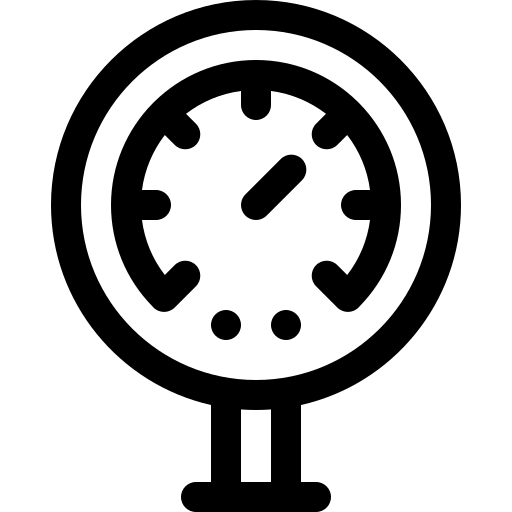
\includegraphics[width=0.5cm]{PressureGuageIcon.png}};
  \node at (1,0.91) {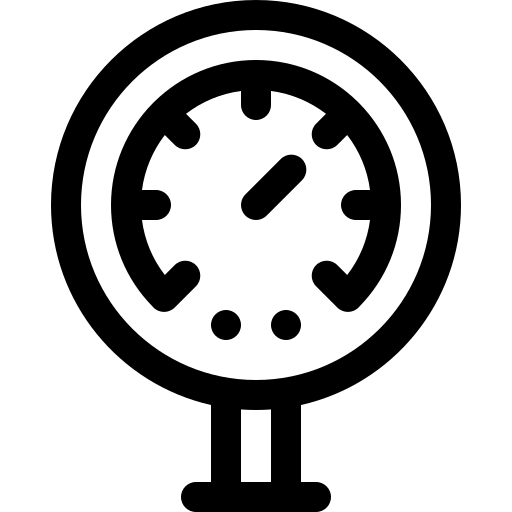
\includegraphics[width=0.5cm]{PressureGuageIcon.png}};

\draw (0,0) .. controls (0.98,1.05) and (1.02,1.05) .. (2,0);
\draw (1.1,1.05) node[anchor=north west] {$Pressure=62psi$};
\draw (-0.65,0.5) node[anchor=north east] {$Flow=120 gpm$};
\draw (-0.65,0.3) node[anchor=north east] {$Pressure=100psi$};
\end{tikzpicture}\\
\vspace{0.2cm}
Total headloss = Headloss due to elevation gain + Headloss due to friction\\
\vspace{0.2cm}
$\implies$ Headloss due to friction = Total headloss - Headloss due to elevation gain\\
\vspace{0.2cm}
Total headloss = $(100 - 62)\enspace \cancel{psi}* \dfrac{ft \enspace head}{0.433\cancel{psi}}=87.8 ft $\\
Headloss due to elevation gain = $60 \enspace ft $\\
$\implies$ Headloss due to friction = $87.8-60=\boxed{27.8 \enspace ft}$\\
\vspace{0.2cm}
\end{enumerate}




\section*{Practice Problems - Pumping Power Requirements} \index{Math solutions!Pumping power requirements}
\begin{enumerate}

\item If a pump is operating at 2,200 gpm and 60 feet of head, what is the water horsepower? If the pump efficiency is 71\%, what is the brake horsepower?\\
\vspace{0.2cm}
Solution:\\
\vspace{0.2cm}
water Hp = flow * head\\
$2,200GPM*60ft*\dfrac{Hp}{3,960 GPM-ft}=\boxed{Water \enspace Hp = 33.3Hp}$\\
\vspace{0.4cm}
pump Hp = brake Hp * pump efficiency\\
$brake \enspace Hp = \dfrac{33.3}{0.71}=\boxed{Brake \enspace Hp=47Hp}$
 \vspace{0.2cm}


\item The water horsepower of a pump is $10 \mathrm{Hp}$ and the brake horsepower output of the motor is $15.4 \mathrm{Hp}$. What is the efficiency of the pump?\\
\vspace{0.2cm}
Solution:\\ 
 \vspace{0.2cm}
 \vspace{0.4cm}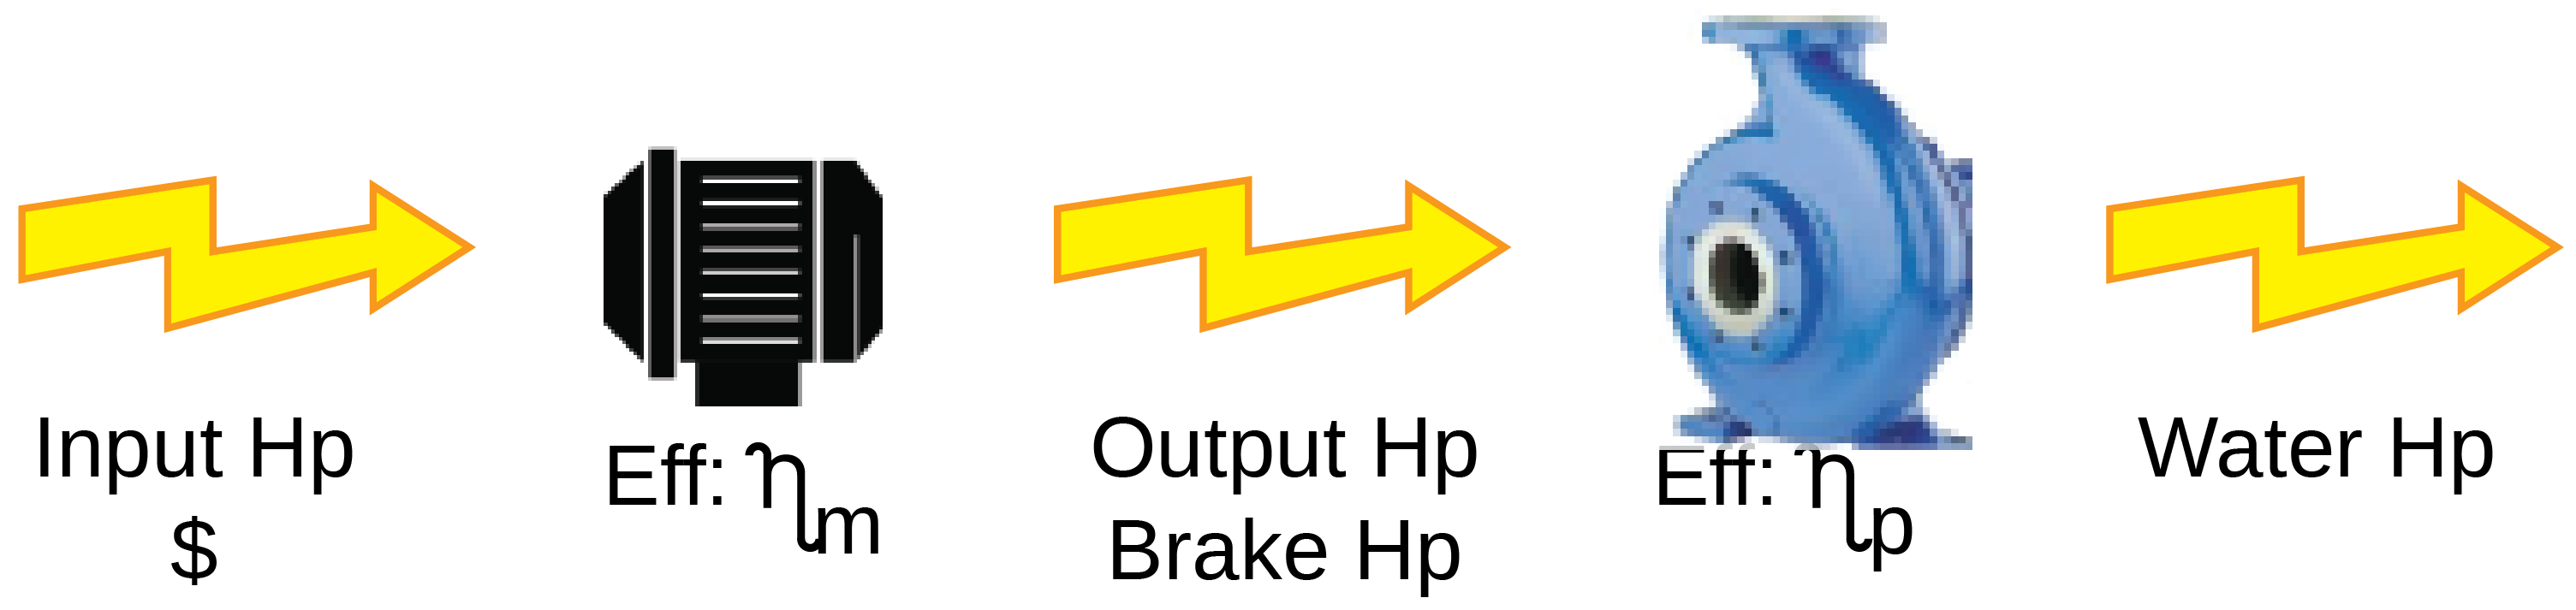
\includegraphics[scale=0.08]{PumpProblem}\\
 \vspace{0.2cm}
 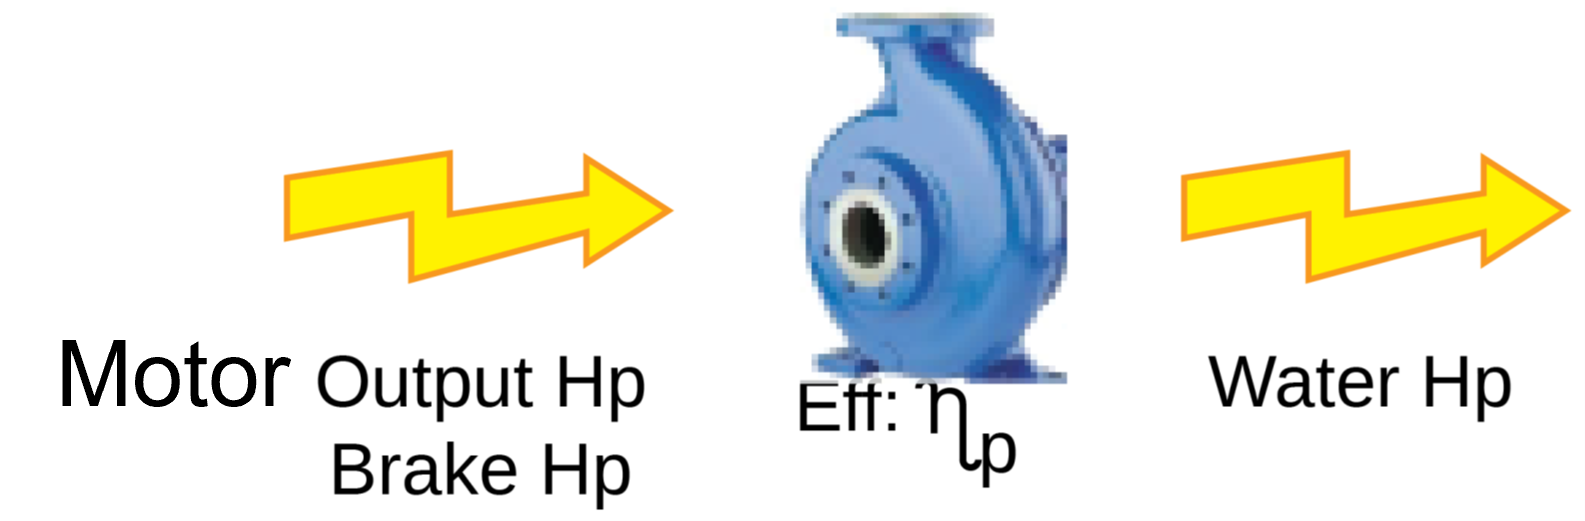
\includegraphics[scale=0.32]{PumpingProblemPump}
 $\eta_p=\dfrac{10 \mathrm{BHp}}{15.4 \mathrm{EHp}} \times 100=\boxed{65 \%}$\\
 \vspace{0.2cm}
 
 \item The water horsepower of a pump is $25 \mathrm{Hp}$ and the brake horsepower output of the motor is $48 \mathrm{Hp}$. What is the efficiency of the pump?\\
 Solution:\\
  \vspace{0.2cm}
 \vspace{0.32cm}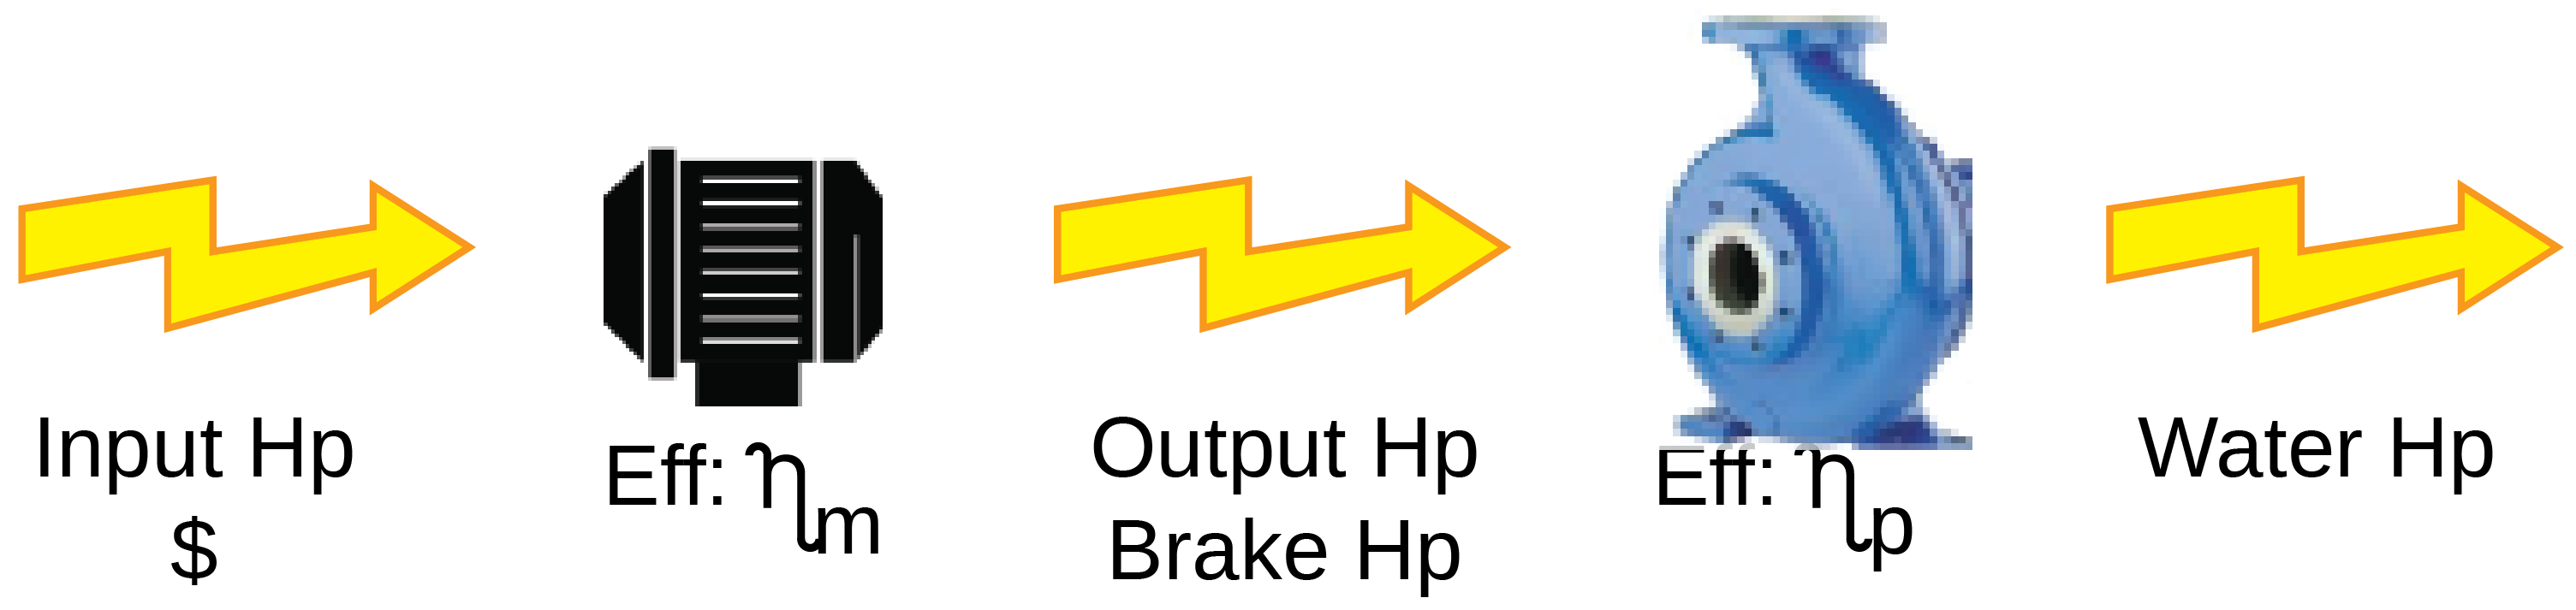
\includegraphics[scale=0.08]{PumpProblem}\\
 \vspace{0.2cm}
 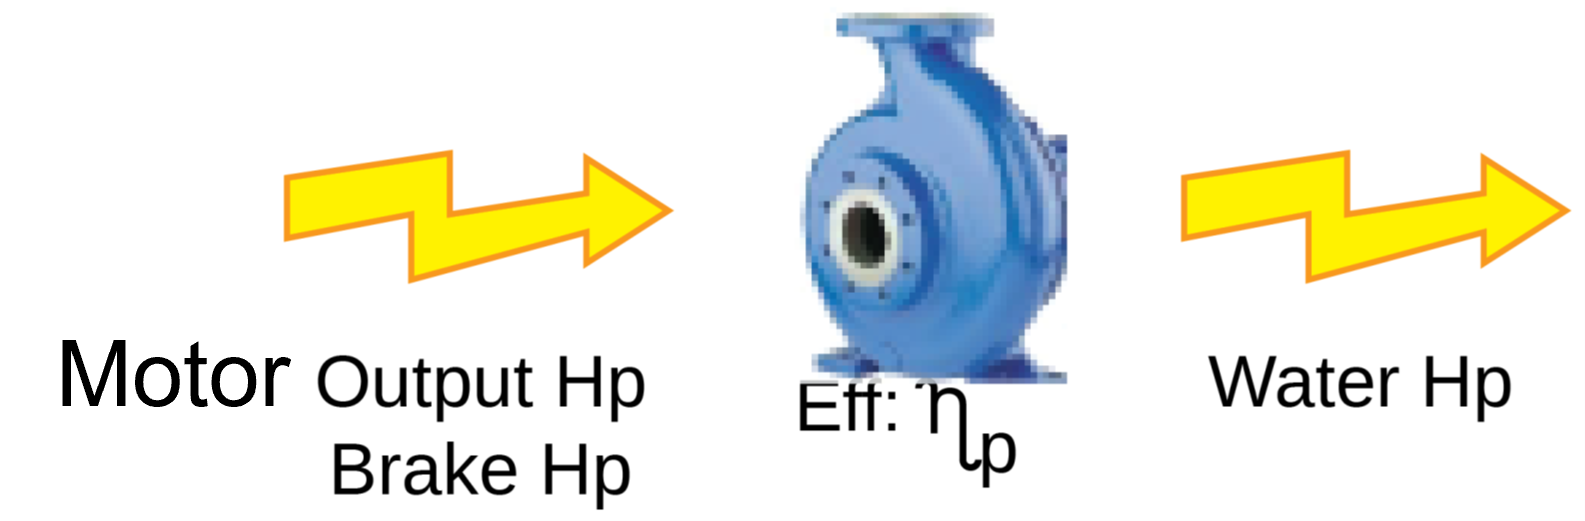
\includegraphics[scale=0.4]{PumpingProblemPump}
 \vspace{0.2cm}
$\eta_p=\dfrac{25 \mathrm{\enspace Water \enspace Hp}}{48 \mathrm{\enspace brake \enspace Hp}} \times 100=\boxed{52 \%}$
  \vspace{0.4cm}

\item The efficiency of a well pump is determined to be $75 \%$. The efficiency of the motor is estimated at $94 \%$. What is the efficiency of the well?\\
 \vspace{0.2cm}
Solution:\\ 
 \vspace{0.2cm}
$Well \enspace efficiency=\eta_m * \eta_p \implies 0.94 \times 0.75=0.705 \times 100=\boxed{71 \%}$
 \vspace{0.2cm}

 \item If a motor is $85 \%$ efficient and the output of the motor is determined to be 10 $\mathrm{BHp}$, what is the electrical horsepower requirement of the motor?
 \vspace{0.2cm}
Solution:\\ 
 \vspace{0.2cm}
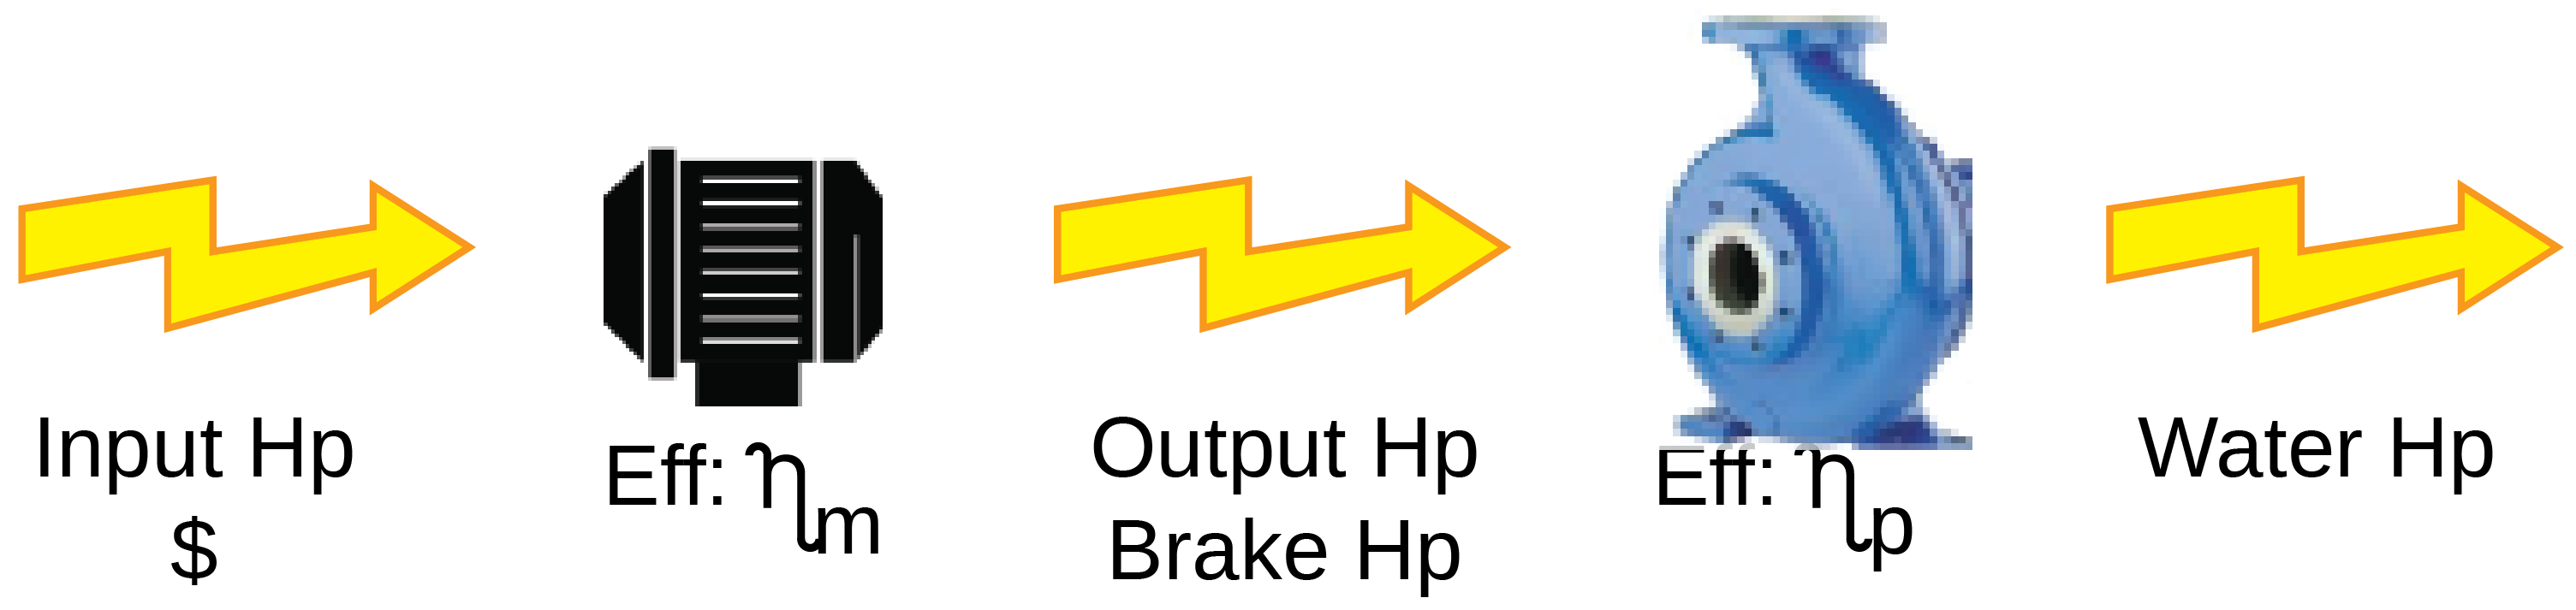
\includegraphics[scale=0.08]{PumpProblem}\\
 \vspace{0.2cm}
 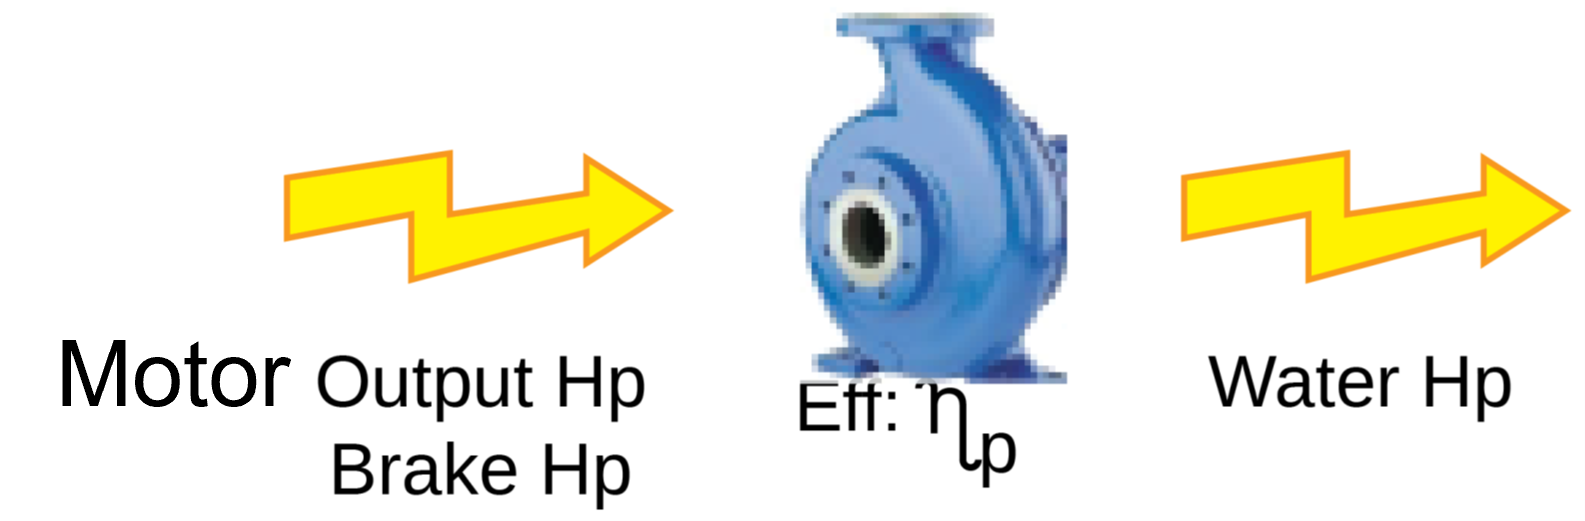
\includegraphics[scale=0.32]{PumpingProblemPump}\\
 \vspace{0.2cm}
$\dfrac{10 \mathrm{BHp}}{0.85}=\boxed{11.8 \mathrm{EHp \enspace or \enspace Input \enspace Hp}}$
 \vspace{0.2cm}

\item The water horsepower of a well with a submersible pump has been calculated at 8.2 WHp. The Output of the electric motor is measured as $10.3 \mathrm{BHp}$. What is the efficiency of the pump?\\
 \vspace{0.2cm}
Solution:\\ 
 \vspace{0.2cm}
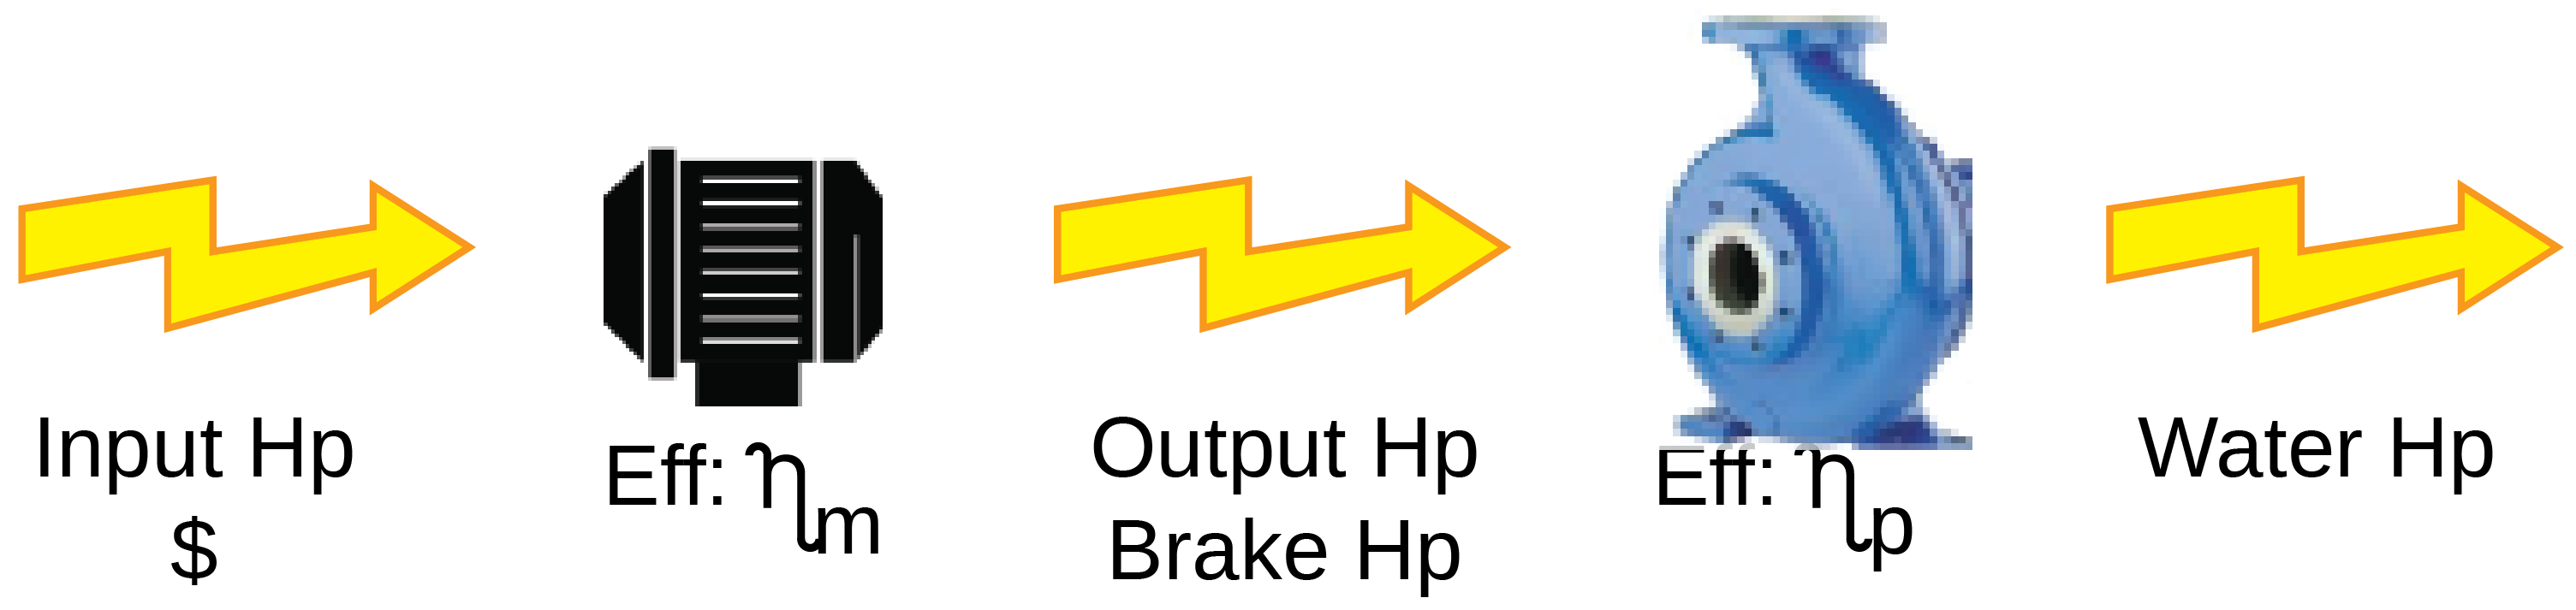
\includegraphics[scale=0.08]{PumpProblem}\\
 \vspace{0.2cm}
 \includegraphics[scale=0.32]{PumpingProblempump}\\
 \vspace{0.2cm}
$\eta_p=\dfrac{82 \mathrm{\enspace W \enspace Hp}}{10.3 \mathrm{\enspace BHp}} \times 100=\boxed{79.6 \%}$
 \vspace{0.2cm}
 
 \vspace{0.2cm}


   \item Water is being pumped from a reservoir to a storage tank on a hill. The elevation difference between water levels is 1200 feet. Find the pump size (in Hp) required to fill the tank at a rate of 120 gpm.\\
  \vspace{0.2cm}
\begin{tikzpicture}[scale=1]
\draw (0,0) .. controls (1.98,3.5) and (2.02,3.5) .. (4,0);
\node[cylinder, 
    draw = violet, 
    text = purple,
    cylinder uses custom fill, 
    cylinder body fill = blue!10, 
    cylinder end fill = magenta!40,
    aspect = 0.1, 
    shape border rotate = 90] (c) at (2,3.0) {Storage};
\node[cylinder, 
    draw = violet, 
    text = purple,
    cylinder uses custom fill, 
    %cylinder body fill = magenta!10, 
    %cylinder end fill = magenta!40,
    minimum size = 0.3cm, aspect = 0.1,
    shape border rotate = 90] (c) at (2,3.5) {\hspace{0.25cm}{Water}\hspace{0.25cm}};

  \node at (-3,0.1) {\includegraphics[width=3cm]{PumpIcon.png}};
   \node at (-3,-0.8) {
\includegraphics[width=2cm]{WaterReservoirIcon.png}};
   
\draw [ultra thick, -] (-3,-.9) -- (-3,0) node [midway, below] {};
\draw [ultra thick, -] (-3.28,0.63) -- (-3.28,3.1) node [midway, below] {};
\draw [ultra thick, ->] (-3.28,3.1) -- (1.2,3.1) node [midway, below] {};
\draw [ultra thick, ->] (-3.28,3.1) -- (1.2,3.1) node [midway, below] {};
\draw[dashed] (-1.8,-1) -- (2.5,-1);
\draw [<->] (2,-1) -- (2,3.25) node [midway, below] {\hspace{5cm}Elevation difference = 1200 ft};
\draw (0.5,3.7) node[anchor=north east] {$Flow = 120 gpm$};
\end{tikzpicture}\\
\vspace{0.2cm}
Solution:\\
\vspace{0.2cm}
water Hp = flow * head\\
$120GPM*1,200ft*\dfrac{Hp}{3,960 GPM-ft}=\boxed{Water \enspace Hp = 36.4Hp}$\\


\end{enumerate}

\section*{Practice Problems - Well Hydraulics}\index{Math solutions!Well hydraulics}

\begin{enumerate}


\item A well yields 2,840 gallons in exactly 20 minutes. What is the well yield in gpm?\\
Solution:\\
\vspace{0.2cm}
$\dfrac{2,840gal}{20min}=\boxed{142\dfrac{gal}{min}}$


\vspace{0.2cm}
\item Before pumping, the water level in a well is 15 ft. down. During pumping, the water level is 45 ft. down. The drawdown is:\\
Solution:\\
\vspace{0.2cm}
$45-15=\boxed{30 ft}$


\vspace{0.2cm}
\item A well is located in an aquifer with a water table elevation 20 feet below the ground surface. After operating for three hours, the water level in the well stabilizes at 50 feet below the ground surface. Calculate the pumping water level.\\
Solution:\\
\vspace{0.2cm}
$\boxed{50ft}$


\vspace{0.2cm}
\item Calculate drawdown, in feet, using the following data:\\
The water level in a well is 20 feet below the ground surface when the pump is not in operation, and the water level is 35 feet below the ground surface when the pump is in operation.\\
Solution:\\
\vspace{0.2cm}

  $\text {Drawdown} = 35 \mathrm{ft}-20 \mathrm{ft}=\boxed{15ft}$\\


\vspace{0.2cm}
\item Calculate the well yield in gpm, given a drawdown of 14.1 ft and a specific yield of 31 gpm/ft.\\
Solution:\\
\vspace{0.2cm}
  $Specific \enspace Yield \enspace(gpm/ft) =\dfrac{ Yield \enspace(gpm)}{ Drawdown \enspace(ft)}$\\
  \vspace{0.2cm}

  $\implies Yield \enspace(gpm) = Specific \enspace Yield \enspace(gpm/ft)*Drawdown \enspace(ft)=31*14.1=\boxed{437.1 \enspace gpm}$

\end{enumerate}

\section*{Practice Problems - Sedimentation} \index{Math solutions!Sedimentation}

\begin{enumerate}

\item Calculate the detention time for a sedimentation tank that is 48 feet wide, 210 feet long and 9 feet deep with a flow of 5 MGD.\\

\vspace{0.5cm}

Solution: \\
$Clarifier \enspace detention \enspace time \enspace (hr) = 	\dfrac{ Clarifier \enspace volume (cu.ft \enspace or \enspace gal)}{Influent \enspace flow \enspace (cu.ft \enspace or \enspace gal)/hr)}$\\
$Clarifier \enspace detention \enspace time \enspace (hr) = 	\dfrac{(48*210*9)\cancel{ft^3}}{\dfrac{5\cancel{MG}}{\cancel{day}}*\dfrac{10^6\cancel{gal}}{\cancel{MG}}*\dfrac{\cancel{ft^3}}{7.48\cancel{gal}}*\dfrac{\cancel{day}}{24hrs}}=\boxed{3.25hrs}$\\



\item  At a 2.5 MGD wastewater treatment plant the primary clarifier has a detention time of 2 hours. How many gallons does this clarifier hold?\\

\vspace{0.5cm}
Solution:\\
\vspace{0.2cm}
$Clarifier \enspace detention \enspace time \enspace (hr) = 	\dfrac{ Clarifier \enspace volume (gal)}{Influent \enspace flow \enspace (gal/hr)}$\\
\vspace{0.2cm}
$ \implies Clarifier \enspace volume (gal)=Clarifier \enspace detention \enspace time \enspace (hr)*Influent \enspace flow \enspace (gal/hr)$\\
\vspace{0.2cm}
$ \implies Clarifier \enspace volume (gal)= \Big(2 \enspace hrs\Big)*\Big(2.5*10^6 \enspace \dfrac{gal}{day}*\dfrac{day}{24 \enspace hrs}\Big)=\boxed{208,333 \enspace gals}$\\



\vspace{0.5cm}

\item A circular clarifier has a diameter of 80 ft. If the flow to the clarifier is 1800 gpm, what is the surface overflow rate in gpm/ft?\\
\vspace{0.2cm}
Solution:\\

$\mathrm{Surface \enspace overflow \enspace rate}=\dfrac{\mathrm{Flow, \enspace gpm}}{\mathrm{Clarifier \enspace surface \enspace area, \enspace ft}^2}=\dfrac{1,800 \enspace \mathrm{gpm}}{(0.785*80^2 )\mathrm{ft}^2}=\boxed{0.36 \enspace \mathrm{gpm/ft}^2}$

\vspace{0.2cm}
\item A sedimentation basin 70 ft by 25 ft receives a flow of 1000 gpm. What is the surface overflow rate in gpm/ft$2$?\\
\vspace{0.2cm}
Solution:\\
$\mathrm{Surface \enspace overflow \enspace rate}=\dfrac{\mathrm{Flow, \enspace gpm}}{\mathrm{Clarifier \enspace surface \enspace area, \enspace ft}^2}=\dfrac{1,000 \enspace \mathrm{gpm}}{(70 \mathrm{ft} \enspace * 25 \mathrm{ft})\mathrm{ft}^2}=\boxed{0.6 \enspace \mathrm{gpm/ft}^2}$

\vspace{0.2cm}

\item A circular clarifier receives a flow of 3.55 MGD. If the diameter of the weir is 90 ft, what is the weir loading rate in gpm/ft?\\

\vspace{0.2cm}
Solution\\

$\mathrm{Weir \enspace overflow \enspace rate}=\dfrac{\mathrm{Flow, \enspace gpm}}{\mathrm{Weir} \enspace \mathrm{length} \enspace ft}$\\
\vspace{0.3cm}
$\implies \dfrac{ \dfrac{3.55 \enspace \mathrm{MG}}{\mathrm{day}}*\dfrac{1,000,000 \enspace \mathrm{gal}}{\mathrm{MG}}*\dfrac{\mathrm{day}}{1440 \enspace \mathrm{min}}}{ (3.14*90) \enspace \mathrm{ft}}=\boxed{2,465 \enspace  \mathrm{gpm/ft}}$\\
\vspace{0.3cm}
\textit{Note: The concentration and volume (or flow) units need to be the same.  Thus, the gpm flow rate of Line 1 was converted to math the MGD flow rate unit of Line 2.}


\end{enumerate}

\section*{Practice Problems - Filtration} \index{Math solutions!Filtration}


\begin{enumerate}
	\item At an average flow of 4,000 gpm, how long of a filter run in hours would be required to produce 25 MG of filtered water?\\
	\vspace{0.2cm}
	\textbf{Solution}\\
	
	$Flow \enspace rate \enspace (gpm)=\dfrac{Total \enspace flow \enspace (gal)}{Filter \enspace run \enspace time \enspace (min)}$

\vspace{0.3cm}

$\implies Filter \enspace run \enspace time \enspace (min)=\dfrac{Total \enspace flow \enspace (gal)}{Flow \enspace rate \enspace (gpm)}$\\

\vspace{0.3cm}

$\implies Filter \enspace run \enspace time \enspace (hr)=25 \enspace MG*\dfrac{1,000,000 \enspace \cancel{gal}}{MG}*\dfrac{\cancel{min}}{4,000 \enspace \cancel{gal}}*60 \enspace \dfrac{hr}{\cancel{min}}=\boxed{104 \enspace hrs}$
\vspace{0.3cm}
	
	\item A filter is $40 \mathrm{ft}$ long by $20 \mathrm{ft}$ wide. During a test of flow rate, the influent valve to the filter is closed for 6 minutes. The water level drop during this period is 16 inches. What is the filtration rate for the filter in $\mathrm{gpm} / \mathrm{ft}^{2}$ ?\\
	\vspace{0.2cm}
	\textbf{Solution}\\
	
	$\text{Filtration rate, } \mathrm{gpm} / \mathrm{ft}^{2} = 
\dfrac{(
40 \mathrm{ ft}*20 \mathrm{ ft} * 16 \mathrm{\cancel{in}}*
\dfrac{ft}{12 \enspace \cancel{in}}
)
\cancel{ft^3}*7.48 \enspace 
\dfrac
{gal}
{\cancel{ft^3}}}
{40 \enspace ft * 20 \enspace feet}= \boxed{1.7\enspace gpm/ft^2}$\\
	\vspace{0.3cm}
\item A water treatment plant treats 6.0 MGD with four filters. Each filter use 60,000 gallons per wash. What is the percent backwash at the plant?\\
\vspace{0.2cm}
Solution:\\
\vspace{0.2cm}

Backwash water, $\%=\dfrac{60,000*4 \text { gal }}{6,000,000 \text { gal }} \times 100 = \boxed{4 \%}$\\
\vspace{0.3cm}
\item A treatment plant filter washes at a rate of 10,000 GPM. The filter measures 18ft. wide by 24ft. long. What is the rate of rise expressed in inches per minute?\\
\vspace{0.2cm}
Solution:\\
\vspace{0.2cm}

$$\text{ Backwash rinse rate, in/} \mathrm{min}=\frac{\text { Backwash rate, } \mathrm{gpm} / \mathrm{ft}^{2} \times 12 \mathrm{in} / \mathrm{ft}}{7.48 \mathrm{gal} / \mathrm{ft}^{3}}$$

\textit{Based upon the above formula, the Backwash tate in $gpm/ft^2$ needs to be calculated by dividing the gpm flow by the surface area}

$\text{Backwash Rinse Rate, in/} \mathrm{min}=
\dfrac{\Biggl(\dfrac{10,000 \mathrm{gpm}}{18 \mathrm{ft} \times 24 \mathrm{ft}}\Biggr) \times \dfrac{12 \mathrm{in}}{\mathrm{ft}}
}
{
7.48 \mathrm{gal} / \mathrm{ft}^{3}
}=\boxed{37in/min}$\\
\vspace{0.3cm}
\item If a filter measures 20 feet by 30 feet by 7 foot deep and the backwash flow is $3.5 \mathrm{cuft} / \mathrm{sec}$, what is the backwash rate?\\
\vspace{0.2cm}
Solution:\\
\vspace{0.2cm}
Backwash Rate (gpm/sq.ft)=$\dfrac{\dfrac{3.5 \enspace ft^3}{sec}*\dfrac{7.48 \enspace gal}{ft^3}*\dfrac{60 \enspace sec}{min}}{(20*30) \enspace ft^2}=\boxed{\dfrac{2.6 \enspace gpm}{ft}}$

\end{enumerate}
